\documentclass[letterpaper,8pt]{extarticle}

% -----------------------
% Package Imports
% -----------------------
\usepackage{amssymb,amsmath,amsthm,amsfonts}
\usepackage{multicol,multirow}
\usepackage{calc}
\usepackage{ifthen}
\usepackage[landscape]{geometry}
\usepackage{array}% http://ctan.org/pkg/array
\usepackage{enumitem}% http://ctan.org/pkg/enumitem
\usepackage[colorlinks=true,citecolor=blue,linkcolor=blue]{hyperref}
\usepackage{booktabs}
\usepackage{bookmark}
\usepackage[normalem]{ulem}
\usepackage{enumitem}
\usepackage{ragged2e}
\usepackage{graphicx}
\usepackage{siunitx}
\usepackage{tikz}
\usetikzlibrary{shapes.geometric, arrows}
\usetikzlibrary{arrows.meta, positioning}
\usepackage{derivative}
\usepackage{svg}
\usepackage{listings}
\usepackage{setspace}
\usepackage{xcolor}
\usepackage{courier}
\usepackage{syntax}
\usepackage{mathpartir}
\usepackage{courier}
\usepackage{vwcol}
\usepackage{xcolor}

\usepackage[sfdefault,lf]{carlito}
\renewcommand{\familydefault}{\sfdefault}

\usepackage[T1]{fontenc}   % Use T1 encoding to access full font
\usepackage{tgcursor}

\definecolor{dkgreen}{rgb}{0,0.6,0}
\definecolor{gray}{rgb}{0.5,0.5,0.5}
\definecolor{mauve}{rgb}{0.58,0,0.82}

\definecolor{background}{HTML}{f8f1e6}
\definecolor{h1}{HTML}{135b20}
\definecolor{h2}{HTML}{2b8854}
\definecolor{h3}{HTML}{bd6b11}
\definecolor{h4}{HTML}{a48758}
\definecolor{body}{HTML}{000000}

\lstset{
  frame=tb,
  language=python,
  aboveskip=1mm,
  belowskip=1mm,
  showstringspaces=false,
  columns=flexible,
  basicstyle=\ttfamily\tiny,
  numbers=none,
  numberstyle=\tiny\color{gray},
  keywordstyle=\color{blue},
  commentstyle=\color{dkgreen},
  stringstyle=\color{mauve},
  breaklines=true,
  breakatwhitespace=true,
  tabsize=3
}

% -----------------------
% Definitions
% -----------------------
\newcommand{\definition}[2]{
  % Start a new paragraph
  \hangindent=1em
  \textbf{#1}: #2%
}

% -----------------------
% Subtitle
% -----------------------
\newcommand{\subtitle}[2]{
  % Start a new paragraph
  \hangindent=1em
  \textbf{\color{h4}#1 | #2}\\
  \hrulefill
}
% -----------------------
% Geometry settings (minimal margins)
% -----------------------
\geometry{top=0.25in, left=0.25in, right=0.25in, bottom=0.35in}

% -----------------------
% Environment for Figures in multicolumn layouts
% -----------------------
\newenvironment{Figure}
{\par\medskip\noindent\minipage}
{\endminipage\par\medskip}

\pagestyle{empty} % remove page numbers

% -----------------------
% Section formatting (make things more compact)
% -----------------------
\makeatletter
\renewcommand{\section}{\@startsection{section}{1}{0mm}%
  {-1ex plus -0.5ex minus -0.2ex}%
  {0.5ex plus 0.2ex}%
{\color{h1} \normalfont\small\bfseries}}
\renewcommand{\subsection}{\@startsection{subsection}{2}{0mm}%
  {-1ex plus -0.5ex minus -0.2ex}%
  {0.5ex plus 0.2ex}%
{\color{h2}\normalfont\fontsize{6}{6}\selectfont\bfseries}}
\renewcommand{\subsubsection}{\@startsection{subsubsection}{3}{0mm}%
  {-1ex plus -0.5ex minus -0.2ex}%
  {1ex plus 0.2ex}%
{\color{h3} \normalfont\fontsize{5.5}{5.5}\selectfont\bfseries\itshape}}
\makeatother
\setcounter{secnumdepth}{0} % disable section numbering

\setlength{\lineskip}{0pt}  % Reduces space between lines
\setlength{\lineskiplimit}{0pt}

% -----------------------
% Spacing adjustments
% -----------------------
% \setlength{\parindent}{0pt}
% \setlength{\parskip}{0pt plus 0.5ex}

% -----------------------
% Custom Commands and Shorthands
% -----------------------
\DeclareSIUnit\noop{\relax}

\newcommand{\To}{\Rightarrow}
\newcommand{\ttt}{\texttt}
\newcommand{\ra}{\rightarrow}

\newcommand{\bul}[1]{%
  \par\hangindent=1.5em\hangafter=1
  \noindent\hspace*{0.25em}\scalebox{0.7}{$\bullet$}\hspace{0.5em}%
  \hyphenpenalty=10000\RaggedRight{}#1\par\vspace{0.3ex}%
}

\newcommand{\divider}{
  \vskip\medskipamount % or other desired dimension
  \leaders\vrule width \textwidth\vskip{0.4pt} % or other desired thickness
  \vskip\medskipamount % ditto
  \nointerlineskip
}

% -----------------------
% Condense itemize and enumerate environments
% -----------------------
\let\olditemize\itemize \let\endolditemize\enditemize
\renewenvironment{itemize}{\olditemize \itemsep0em}{\endolditemize}
\let\oldenumerate\enumerate \let\endoldenumerate\endenumerate
\renewenvironment{enumerate}{\oldenumerate \itemsep0em}{\endoldenumerate}
\setlist[itemize]{noitemsep, topsep=0pt, leftmargin=*}
\setlist[enumerate]{noitemsep, topsep=0pt,  leftmargin=*}

\let\oldtabular\tabular \let\oldendtabular\endtabular
\renewenvironment{tabular}[1]{%
  \hyphenpenalty=10000\RaggedRight{}
  \hbadness=10000\relax
  \oldtabular{#1}%
}{%
  \oldendtabular
}

\usepackage{etoolbox}
\AtBeginEnvironment{align*}{\vspace{-0.2cm}}
\AtEndEnvironment{align*}{\vspace{-0.7em}}

% -----------------------
% Title / Header
% -----------------------
\date{}

\begin{document}
\pagecolor{background}
\color{body}

\raggedright
\tiny

% -----------------------
% Listings settings (for code snippets)
% -----------------------

\begin{center}
  {\textbf{Networks Design Notes} - {Elite Lu}}
\end{center}

\setlength{\tabcolsep}{2pt}
\renewcommand{\arraystretch}{1.2}

% -----------------------
% Adjust Column Spacing for Multicolumn Layout
% -----------------------
\setlength{\premulticols}{1pt}
\setlength{\postmulticols}{1pt}
\setlength{\multicolsep}{1pt}
\setlength{\columnsep}{2pt}

\title{Networks Design Notes}
\author{Elite Lu}

\begin{multicols*}{5}

  \begin{center}
    
\includegraphics[width=4.8cm]{ROWLET.png}
  \end{center}

  \section{Abbreviations and Acronyms}

  \begin{multicols*}{2}
    \definition{2oo2}{Two out of Two}

    \definition{2oo3}{Two out of Three}

    \definition{3GPP}{3rd Generation Partnership Project}

    \definition{3oo3}{Three out of Three}

    \definition{ACE}{Axle Counter Evaluator}

    \definition{ACE}{Access Control List}

    \definition{AP}{Access Point}

    \definition{API}{Application Program Interface}

    \definition{ASK}{Amplitude Shift Keying}

    \definition{BFD}{Bi-directional Forwarding Detection}

    \definition{BPSK}{Binary Phase Shift Keying}

    \definition{B}{Business (Used in X2X)}

    \definition{C}{Consumer (Used in X2X)}

    \definition{CP}{Control Plane}

    \definition{CBTC}{Communications-Based Train Control}

    \definition{CBRS}{Citizens Broadband Radio Service (150 MHz wideband of 3.5 GHz band)}

    \definition{Cisco FM}{Cisco Fluidmesh}

    \definition{CLI}{Command Line Interface}

    \definition{COTS}{Commercial Off-The-Shelf}

    \definition{CPU}{Central Processing Unit}

    \definition{CRC}{Cyclic Redundancy Check}

    \definition{CSMA}{Carrier Sense Multiple Access}

    \definition{CSMA/CA}{Carrier Sense Multiple Access with Collision Avoidance}

    \definition{DDoS}{Distributed Denial of Service}

    \definition{DF}{Don't Fragment}

    \definition{FCAPS}{Fault, Configuration, Accounting, Performance, Security}

    \definition{FDM}{Frequency Division Multiplexing}

    \definition{FSK}{Frequency Shift Keying}

    \definition{FTTH}{Fiber-To-The-Home}

    \definition{G}{Government (Used in X2X)}

    \definition{gNB}{Next Generation Node B}

    \definition{MAC}{Medium Access Control/Media Access Control}

    \definition{MF}{More Fragments}

    \definition{OFDM}{Orthogonal Frequency Division Multiplexing}

    \definition{OS}{Operating System}

    \definition{OSI}{Open Systems Interconnection}

    \definition{OSS}{Operational Support Systems}

    \definition{P}{Peer (Used in X2X)}

    \definition{POP}{Point of Presence}

    \definition{PSK}{Phase Shift Keying}

    \definition{QNS}{Qualitative Numerical Data}

    \definition{QoS}{Quality of Service}

    \definition{QUIC}{Quick UDP Internet Connections}

    \definition{RRD}{Round-Robin-Database}

    \definition{RFID}{Radio Frequency Identification}

    \definition{RR}{Resource Record}

    \definition{RTT}{Round Trip Time}

    \definition{RW}{Read \& Write}

    \definition{SA}{Standalone Deployment}

    \definition{SMB}{Server Message Block}

    \definition{STP}{Shield Twisted Pair}

    \definition{TDM}{Time Division Multiplexing}

    \definition{TTL}{Time To Live}

    \definition{UTP}{Unshielded Twisted Pair}

  \end{multicols*}

  \subsection{Corporations and Entities}

  \definition{ANSI}{American National Standards Institute}

  \definition{AREMA}{American Railway Engineering and Maintenance-of-Way Association}

  \definition{CENELEC}{European Committee for Electromechanical Standardization}

  \definition{IEEE}{Institute of Electrical and Electronics Engineers}

  \definition{ITU}{International Telecommunications Union}

  \subsection{Files}

  \begin{multicols*}{2}

    \definition{CSS}{Cascading Style Sheets}

    \definition{HTML}{Hyper Text Markup Language}

    \definition{JPEG/JPG}{Joint Photographic Experts Group}

    \definition{JMX}{Java Management Extensions (APIs)}

    \definition{MP3}{MPEG Audio Layer 3}

  \end{multicols*}

  \subsection{Internet and Websites}

  \begin{multicols*}{2}

    \definition{DNS}{Domain Name System}

    \definition{ISP}{Internet Service Provider}

    \definition{TLD}{Top-Level Domain}

    \definition{URL}{Uniform Resource Locator}

    \definition{W3C}{World Wide Web Consortium (www)}

  \end{multicols*}

  \subsection{Networks}

  \begin{multicols*}{2}

    \definition{5GC}{5G Core Network}

    \definition{AMF}{Access and Mobility Management Function}

    \definition{G}{Generation (Used in Cellular)}

    \definition{gNB}{5G NR Radio Base Station}

    \definition{LAN}{Local Area Network (Building)}

    \definition{LTE}{Long Term Evolution}

    \definition{MAN}{Metropolitan Area Network (City)}

    \definition{MNO}{Mobile Network Operator}

    \definition{NAT}{Network Address Translation}

    \definition{NIC}{Network Interface Card}

    \definition{NSP}{Network Service Provider}

    \definition{PAN}{Personal Area Network (Vicinity)}

    \definition{PDN}{Packet Data Networks}

    \definition{VLAN}{Virtual Local Area Network}

    \definition{VPN}{Virtual Private Network (WAN)}

    \definition{WAN}{Wide Area Network (Country)}

    \definition{Wi-Fi}{Wireless-Fidelity}

    \definition{WPA2}{Wi-Fi Protected Access II}

    \definition{WLAN}{Wireless Local Access Network}

    \definition{WWAN}{Wireless Wide Area Network}

  \end{multicols*}

  \subsection{Protocols}

  \begin{multicols*}{2}

    \definition{ARP}{Address Resolution Protocol}

    \definition{ATS}{Automatic Resolution Protocol}

    \definition{BGP}{Border Gateway Protocol}

    \definition{BPDU}{Bridge Protocol Data Units}

    \definition{DHCP}{Dynamic Host Configuration Protocol}

    \definition{HTTP}{Hypertext Transfer Protocol}

    \definition{HTTPS}{Hypertext Transfer Protocol Secure}

    \definition{ICMP}{Internet Control Message Protocol}

    \definition{IMAP}{Internet Message Access Protocol}

    \definition{IP}{Internet Protocol}

    \definition{IPsec}{Internet Protocol Security}

    \definition{MRP}{Media Redundancy Protocol}

    \definition{NTP}{Network Time Protocol}

    \definition{POP3}{Post Office Protocol version 3}

    \definition{RSTP}{Rapid Spanning Tree Protocol}

    \definition{SCEP}{Simple Certificate Enrollment Protocol}

    \definition{SFTP}{Secure File Transfer Protocol}

    \definition{SMTP}{Simple Mail Transfer Protocol}

    \definition{SNMP}{Simple Network Management Protocol}

    \definition{SNTP}{Simple Network Time Protocol}

    \definition{TCP}{Transmission Control Protocol}

    \definition{UDP}{User Datagram Protocol}

  \end{multicols*}

  \subsubsection{TCP Flags}

  \begin{multicols*}{2}

    \definition{ACK}{Acknowledge}

    \definition{CWR}{Congestion Window Reduced}

    \definition{ECE}{Explicit Congestion Notification Echo}

    \definition{FIN}{Finish}

    \definition{PSH}{Push}

    \definition{RST}{Reset}

    \definition{SYN}{Synchronize}

    \definition{URG}{Urgent}

  \end{multicols*}

  \section{General Definitions}

  \definition{Client}{A device or software application that requests services or resources from a server.}

  \definition{Daemon}{A background program or process that runs independently on a computer system to perform tasks or provide services. Named after Greek mythology's interpretation of a daemon as a mythical being working in the background.}

  \definition{Demultiplexing}{The process of separating a combined stream or signal into individual parts. This is done at each layer, where the TCP/UDP port is used in level 4, IP for level 3, MAC address for level 2.}

  \definition{Flat Structure}{Minimal or no middle management layers, with few hierarchical levels between employees and executives}

  \definition{Frequency Division Multiplexing}{Where different channels are transmitted in different frequency bands.}

  \definition{Host}{A device that can send or receive traffic.}

  \definition{Internet}{A set of all connected networks (Planet).}

  \definition{Multiplexing}{The process of sending multiple signals or streams in a single complex stream. A TCP/UDP port is assigned and added to the stream, along with other headers and the application data.}

  \definition{Network}{A group of interconnected nodes/hosts that transports traffic between them}

  \definition{Network Linking Device}{Any hardware that connects different network resources. This includes switches, routers, bridges, etc.}

  \definition{Process}{A program that runs within the end host. The client starts the communication and the server waits for contact.}

  \definition{Protocol}{Denotes how service implementation is carried out.}

  \definition{Server}{A powerful computer or system that provides services and resources to other computers on a network, called clients.}

  \definition{Service}{What a layer does (IP, TCP, etc.)}

  \definition{Service Interface}{Denotes the means of access (e.g. Socket interface).}

  \definition{Standalone Deployment}{A system or application that operates independently without relying on other systems or networks for its functionality.}

  \definition{Time Division Multiplexing}{A round-robin multiplexing method where each user periodically gets the entire bandwidth for a little burst of time.}

  \section{Units}

  \begin{multicols*}{2}

    \definition{bps}{Bits per second}

    \definition{dBi}{Decibel Isotropic}

    \definition{dBm}{Decibel Milliwatts}

    \definition{Gbps}{Gigabits per second}

    \definition{Mbps}{Megabits per second}

    \definition{Msec}{Millisecond}

  \end{multicols*}

  \section{Models}
  \begin{multicols*}{2}
    \subsection{OSI}
    \begin{enumerate}
      \item[7.] \textbf{Application}
      \item[6.] \textbf{Presentation}
      \item[5.] \textbf{Session}
      \item[4.] \textbf{Transport}
      \item[3.] \textbf{Network}
      \item[2.] \textbf{Data Link}
      \item[1.] \textbf{Physical}
    \end{enumerate}

    \columnbreak

    \subsection{TCP/IP Model}
    \begin{enumerate}
      \item[4.] \textbf{Application (OSI 5-7)}
      \item[3.] \textbf{Transport(OSI 4)}
      \item[2.] \textbf{Internet (OSI 2 \& 3)}
      \item[1.] \textbf{Network Access (OSI 1)}
    \end{enumerate}

    \textbf{To send data, go from layer 7-1 (multiplexing) \& for receiving data, go from layer 1-7 (demultiplexing).}
  \end{multicols*}

  \section{General Information}

  \subsection{Computer Networks Usage}

  \subsubsection{Business Applications}

  \begin{itemize}
    \item Companies use networks for resource sharing with client-server model
    \item B2B, B2C, G2C, C2C, P2P
  \end{itemize}

  \subsubsection{Home Applications}

  \begin{itemize}
    \item Contains many networked devices (computers, home phones, etc.)
    \item No fixed client and servers P2P model
  \end{itemize}

  \subsubsection{Mobile Users}

  \begin{itemize}
    \item Smart devices like phones, smart lights, virtual assistants, etc.
    \item Wireless and mobile related but different
  \end{itemize}

  \subsubsection{Social Issues}

  \definition{Anonymity}{The ability to engage in online activities without revealing your real identity, such as your name, location, or other personally identifiable information.}

  \definition{Censorship}{The legal control or suppression of what can be accessed, published, or viewed on the Internet.}

  \definition{Content Ownership}{The legal and practical right to control how content is used, distributed, and modified.}

  \definition{Data Theft (Theft of Information)}{Refers to the unauthorized acquisition of data or information from an individual, organization, or system.}

  \definition{Piracy}{The illegal copying, distribution, and use of copyrighted material online.}

  \definition{Network Neutrality}{Principle that ISPs should treat all Internet traffic equally, without prioritizing or discriminating against certain content, applications, or services}

  \subsection{IEEE802.11 (Wi-Fi)}

  \begin{itemize}
    \item Clients communicate via an \textbf{AP} that is wired to the rest of the network
    \item Signals in the ISM band can vary in strength due to many effects such as multipath fading due to reflections
    \item Requires complex transmission schemes such as \textbf{OFDM}
    \item Radio broadcasts interfere with each other, so designs such as \textbf{CSMA} are used
  \end{itemize}

  \subsection{Connection-Oriented \& Connectionless}

  \definition{Connection-Oriented}{A connection must be set up for ongoing use (and torn down after use). An example is phone calls.}

  \begin{itemize}
    \item Reliable message stream (Sequence of pages)
    \item Reliable byte stream (Movie download)
    \item Unreliable connection (Voice over IP)
  \end{itemize}

  \definition{Connectionless}{Messages are handled separately. An example is postal service.}

  \begin{itemize}
    \item Unreliable datagram (Junk mail)
    \item Acknowledged datagram (Texting)
    \item Request-reply (Database query)
  \end{itemize}

  \subsection{Service Primitives}

  \begin{itemize}
    \item A service is provided to the layer above as primitives
    \item Primitives are normally system calls
  \end{itemize}

  \begin{center}
    \begin{tabular}{| m{1cm} | m{3.8cm} |}
      \hline
      \textbf{ACCEPT}     & Accept an incoming connection from a peer.         \\
      \hline
      \textbf{CONNECT}    & Established a connection with a waiting peer.      \\
      \hline
      \textbf{DISCONNECT} & Terminate a connection.                            \\
      \hline
      \textbf{LISTEN}     & Block waiting for an incoming \textbf{connection}. \\
      \hline
      \textbf{RECEIVE}    & Block waiting for an incoming \textbf{message}.    \\
      \hline
      \textbf{SEND}       & Send a message to a peer.                          \\
      \hline
    \end{tabular}
  \end{center}

  \subsection{Network Security}

  \begin{center}
    \begin{tabular}{| m{1.1cm} | m{3.7cm} |}
      \hline
      \textbf{DDoS}            & Attackers make resources (server, bandwidth) unavailable for legit traffic by overwhelming resource with bogus traffic.                              \\
      \hline
      \textbf{IP Spoofing}     & Send packet with false source address. Allows for malicious actions without detection.                                                               \\
      \hline
      \textbf{Packet Sniffing} & A network monitoring technique where data packets transmitted across a network are capture and analyzed. A well known software is \textbf{Wireshark} \\
      \hline
      \textbf{Spy Malware}     & Records keystrokes, websites visited, upload info to collection site, etc. Can be enrolled in botnet.                                                \\
      \hline
      \textbf{Virus}           & Self-replicating infection by \textbf{receiving/executing} object that gets itself executed.                                                         \\
      \hline
      \textbf{Worm}            & Self-replicating infection by \textbf{passively receiving} object that gets itself executed.                                                         \\
      \hline
    \end{tabular}
  \end{center}

  \subsection{Network Standardization}

  \begin{center}
    \begin{tabular}{| m{0.5cm} | m{2cm} | m{2.3cm} |}
      \hline
      \textbf{ITU}  & Telecommunications & G.992, ADSL, H.264, MPEG4             \\
      \hline
      \textbf{IEEE} & Communications     & 802.3, Ethernet, 802.11, Wi-Fi        \\
      \hline
      \textbf{IETF} & Internet           & RFC (1034, 1035, 2616), HTTP/1.1, DNS \\
      \hline
      \textbf{W3C}  & Web                & HTML5 standard, CSS standard          \\
      \hline
    \end{tabular}
  \end{center}

  \section{Application Layer}

  \textbf{Data}

  \hrulefill

  \subsection{Mail Access Protocols}

  \begin{center}
    \begin{tabular}{| m{0.5cm} | m{4.3cm} |}
      \hline
      \textbf{SMTP} &
      \bul{Handshake transfer of messages}
      \bul{Used to send emails from one mail server to another}
      \\
      \hline
      \textbf{POP3} &
      \bul{Downloads emails from the server to local device}
      \bul{Downloaded emails are generally unavailable on the server; only available on device}
      \\
      \hline
      \textbf{IMAP} &
      \bul{Allows user to access emails on a server and view on multiple devices}
      \bul{Emails remain on server and changes are synchronized}
      \\
      \hline
    \end{tabular}
  \end{center}

  \subsection{HTTP}

  \begin{itemize}
    \item Webpage consists of objects
    \item Addressable by a single URL with a hostname (www.SOMETHING.idk) and an object pathname (/subdomain/object)
    \item Not specifically for email, but used for accessing web-based email services over the internet
  \end{itemize}

  \subsubsection{Non-Persistent}

  \begin{itemize}
    \item At most one object sent at a time
    \item Requires multiple connections to download multiple objects
    \item Closes the connection after sending a response
    \item \textbf{2 RTTs} for sending each object (\# of RTT = (2 RTT + time to transmit file) $\cdot$ \# of files sent)
  \end{itemize}

  % Diagram
  \begin{center}
    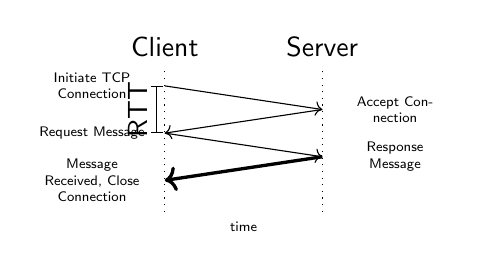
\begin{tikzpicture}[
        every node/.style={transform shape},
        entity/.style={
          rectangle,
          minimum width=1cm,
          minimum height=0.6cm,
          draw,
          align=center,
          font=\scriptsize
        },
        arrow/.style={
          ->,
          thick,
          line width=0.4pt,
          shorten >=1pt,
          shorten <=1pt
        },
        label/.style={
          font=\tiny,
          midway,
          above,
          sloped
        }
      ]

      % Entities
      \node (client) at (-1,0) {Client};
      \node (server) at (1,0) {Server};

      % Timeline
      \draw[dotted] (-1,-2.1) -- (-1,-0.25);
      \draw[dotted] (1,-2.1) -- (1,-0.25);

      % Time labels
      \node[anchor=east, font=\tiny, align=center, text width=1.4cm] at (-1.1,-0.5) {Initiate TCP Connection};
      \node[anchor=west, font=\tiny, align=center, text width=1.4cm] at (1.1,-0.8) {Accept Connection};
      \node[anchor=east, font=\tiny, align=center, text width=1.4cm] at (-1.1,-1.1) {Request Message};
      \node[anchor=west, font=\tiny, align=center, text width=1.4cm] at (1.1,-1.4) {Response Message};
      \node[anchor=east, font=\tiny, align=center, text width=1.4cm] at (-1.1,-1.7) {Message Received, Close Connection};

      \node[anchor=north, font=\tiny, align=center, text width=1.5cm] at (0,-2.1) {time};

      \draw[|-|] (-1.1,-0.5) -- (-1.1, -1.1) node[midway, rotate=90, above] {RTT};

      \draw[->] (-1,-0.5) -- (1, -0.8);
      \draw[->] (1,-0.8) -- (-1, -1.1);
      \draw[->] (-1,-1.1) -- (1, -1.4);
      \draw[->, very thick] (1,-1.4) -- (-1, -1.7);

    \end{tikzpicture}
  \end{center}

  \subsubsection{Persistent}

  \begin{itemize}
    \item Multiple objects can be sent and received with one connection
    \item Leaves the connection open after sending a response
    \item \textbf{1 RTT} for file sending (\# of RTT = 1 RTT for connection + (1 RTT + time to transmit file) $\cdot$ \# of files sent)
  \end{itemize}

  \begin{center}
    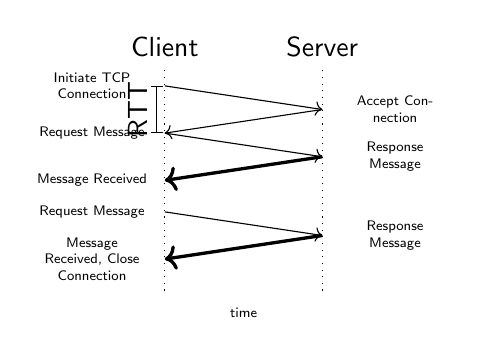
\begin{tikzpicture}[
        every node/.style={transform shape},
        entity/.style={
          rectangle,
          minimum width=1cm,
          minimum height=0.6cm,
          draw,
          align=center,
          font=\scriptsize
        },
        arrow/.style={
          ->,
          thick,
          line width=0.4pt,
          shorten >=1pt,
          shorten <=1pt
        },
        label/.style={
          font=\tiny,
          midway,
          above,
          sloped
        }
      ]

      % Entities
      \node (client) at (-1,0) {Client};
      \node (server) at (1,0) {Server};

      % Timeline
      \draw[dotted] (-1,-3.1) -- (-1,-0.25);
      \draw[dotted] (1,-3.1) -- (1,-0.25);

      % Time labels
      \node[anchor=east, font=\tiny, align=center, text width=1.4cm] at (-1.1,-0.5) {Initiate TCP Connection};
      \node[anchor=west, font=\tiny, align=center, text width=1.4cm] at (1.1,-0.8) {Accept Connection};
      \node[anchor=east, font=\tiny, align=center, text width=1.4cm] at (-1.1,-1.1) {Request Message};
      \node[anchor=west, font=\tiny, align=center, text width=1.4cm] at (1.1,-1.4) {Response Message};
      \node[anchor=east, font=\tiny, align=center, text width=1.4cm] at (-1.1,-1.7) {Message Received};

      \node[anchor=east, font=\tiny, align=center, text width=1.4cm] at (-1.1,-2.1) {Request Message};
      \node[anchor=west, font=\tiny, align=center, text width=1.4cm] at (1.1,-2.4) {Response Message};
      \node[anchor=east, font=\tiny, align=center, text width=1.4cm] at (-1.1,-2.7) {Message Received, Close Connection};

      \node[anchor=north, font=\tiny, align=center, text width=1.5cm] at (0,-3.2) {time};

      \draw[|-|] (-1.1,-0.5) -- (-1.1, -1.1) node[midway, rotate=90, above] {RTT};

      \draw[->] (-1,-0.5) -- (1, -0.8);
      \draw[->] (1,-0.8) -- (-1, -1.1);
      \draw[->] (-1,-1.1) -- (1, -1.4);
      \draw[->, very thick] (1,-1.4) -- (-1, -1.7);
      \draw[->] (-1,-2.1) -- (1, -2.4);
      \draw[->, very thick] (1,-2.4) -- (-1, -2.7);

    \end{tikzpicture}
  \end{center}

  \subsubsection{Request}

  \begin{itemize}
    \item ASCII
    \item Several methods such as GET, POST, etc.
    \item Uploading forms can be done via POST method or URL method
  \end{itemize}

  \textbf{URL Method}

  \begin{itemize}
    \item Used \textbf{GET} method
    \item Inputs are uploaded in the URL fields of the request line, separated with a '?' from the main URL and '\&' between inputs
  \end{itemize}

  \textbf{POST Method}

  \begin{center}
    \begin{tabular}{| m{0.8cm} | m{4cm} |}
      \hline
      \textbf{CONNECT} & Connect through a proxy    \\
      \hline
      \textbf{DELETE}  & Remove a web page          \\
      \hline
      \textbf{GET}     & Read a web page            \\
      \hline
      \textbf{HEAD}    & Read a web page's header   \\
      \hline
      \textbf{OPTIONS} & Query options for a page   \\
      \hline
      \textbf{PUT}     & Store a web page           \\
      \hline
      \textbf{TRACE}   & Echo the incoming response \\
      \hline
    \end{tabular}
  \end{center}

  \subsubsection{Response}

  \begin{center}
    \begin{tabular}{| m{0.4cm} | m{2.1cm} | m{2.1cm} |}
      \hline
      \textbf{1xx} & Informational Response &
      \bul{\definition{100}{Continue}}
      \bul{\definition{101}{Switching Protocols}}
      \\
      \hline
      \textbf{2xx} & Successful             &
      \bul{\definition{200}{OK}}
      \bul{\definition{201}{Created}}
      \bul{\definition{203}{Accepted}}
      \\
      \hline
      \textbf{3xx} & Redirection            &
      \bul{\definition{301}{Moved Permanently}}
      \\
      \hline
      \textbf{4xx} & Client Errors          &
      \bul{\definition{400}{Bad Request}}
      \bul{\definition{401}{Unauthorized}}
      \bul{\definition{402}{Payment Required}}
      \bul{\definition{403}{Forbidden}}
      \bul{\definition{404}{Not Found}}
      \\
      \hline
      \textbf{5xx} & Server Errors          &
      \bul{\definition{502}{Bad Gateway}}
      \bul{\definition{505}{HTTP Version not supported}}
      \\
      \hline
    \end{tabular}
  \end{center}

  \subsection{Web Cache}

  \begin{itemize}
    \item A network entity that satisfies \textbf{HTTP} requests on behalf of the origin Web server
    \item Establishes \textbf{TCP} connection with proxy server
    \item Caches website information to reduce latency, traffic, and response time
    \item Installed by \textbf{ISP}
  \end{itemize}

  \subsection{DNS}

  \begin{itemize}
    \item Internet's "phone book"
    \item Maps \textbf{IP} to names and vice versa
    \item Host aliasing (IP address multiple names, where a complex name can have two simple aliases)
    \item Mail server aliasing, where it translates from a simple alias mail server to its canonical name and its IP address
    \item Load distribution between replicated Web servers (Many IP addresses correspond to one server name)
  \end{itemize}

  \subsubsection{Classes}

  \begin{enumerate}
    \item Root DNS Servers (Around 400 around the world managed by 13 different organizations)
    \item TLD DNS Servers (org, com, edu, etc.)
    \item Authoritative DNS servers (amazon.com, yahoo.com, etc.)
  \end{enumerate}

  To find the IP address of a website:

  \begin{enumerate}
    \item Client queries one of the root servers to find .com DNS servers
    \item Client queries one of the .com DNS servers to get authoritative DNS server
    \item Client queries authoritative DNS server to get IP address
  \end{enumerate}

  \begin{multicols}{2}
    \subsubsection{Types}

    \begin{itemize}
      \item Recursive resolvers
      \item Root nameservers
      \item TLD nameservers
      \item Authoritative nameservers
    \end{itemize}

    \columnbreak

    \subsubsection{Components}

    \begin{itemize}
      \item Domain namespace
      \item Distributed database of name servers
      \item Resolver software that translates domain names into IP addresses
    \end{itemize}
  \end{multicols}

  \subsubsection{Insert Types}

  Also known as \textbf{DNS Record Types}, DNS Insert Types are the different kinds of information stored in the DNS that map domain names to IP addresses.

  \begin{multicols}{2}
    \definition{RR Format}{(Name, Value, Type, TTL)}
    \columnbreak
    \definition{RR Fields}{(NAME, TYPE, CLASS)}
  \end{multicols}

  \begin{center}
    \begin{tabular}{| m{0.8cm} | m{0.8cm} | m{1.0cm} | m{2cm} |}
      \hline
      \textbf{Type}  & \textbf{Type ID} & \textbf{Size}             & \textbf{Description}      \\
      \hline
      \textbf{A}     & 1                & 32 bits                   & Web servers (IPv4)        \\
      \hline
      \textbf{AAAA}  & 28               & 128 bits                  & Web servers (IPv6)        \\
      \hline
      \textbf{CNAME} & 5                & Variable                  & Canonical Domain Name     \\
      \hline
      \textbf{HTTPS} & 65               & 4096 bits                 & HTTPS binding             \\
      \hline
      \textbf{MX}    & 15               & Variable                  & Mail Servers              \\
      \hline
      \textbf{NS}    & 2                & Variable, up to 255 chars & Authoritative Nameservers \\
      \hline
      \textbf{TXT}   & 16               & Variable, up to 255 chars & Text record               \\
      \hline
    \end{tabular}
  \end{center}

  \subsubsection{Inserting Records}

  \begin{enumerate}
    \item Register the name at \textbf{DNS} registrar
    \item Provide the names, the IP addresses of authoritative DNS server (primary and secondary)
    \item Inserts two \textbf{RRs} (type \textbf{NS} and \textbf{A}) into all .com TLD server for both authoritative servers (four records)
  \end{enumerate}

  Note that a \textbf{type A} record for web servers and \textbf{MX} for mail servers need to be created. (https://www.internic.net)

  \begin{multicols}{2}
    \textbf{e.g. elitelu.com}

    Assume that:
    \begin{itemize}
      \item \textbf{dns1.elitelu.com}: 212.221.111.1
      \item \textbf{dns2.elitelu.com}: 212.221.111.2
    \end{itemize}
    \vspace*{\fill}
    \columnbreak

    The final records:

    \begin{itemize}
      \item \textbf{elitelu.com, dns1.elitelu.com, NS}
      \item \textbf{elitelu.com, dns1.elitelu.com, A}
      \item \textbf{elitelu.com, dns2.elitelu.com, NS}
      \item \textbf{elitelu.com, dns2.elitelu.com, A}
    \end{itemize}

  \end{multicols}

  \subsubsection{Vulnerabilities}

  \begin{itemize}
    \item DDoS Attacks
    \item Redirect Attacks (Man in the Middle, DNS poisoning, where bogus replies are sent to DNS server and caches them)
  \end{itemize}

  \section{Presentation}

  \textbf{Data}

  \hrulefill

  \begin{itemize}
    \item Allows applications to interpret data meaning (how data is presented)
    \item Same data can mean different things in different formats
    \item e.g. JPEG, MP3, etc.
  \end{itemize}

  \section{Session}

  \textbf{Data}

  \hrulefill

  \begin{itemize}
    \item Allows applications to maintain ongoing session
    \item Responsible for synchronization, check-pointing, OS, and scheduling
  \end{itemize}

  \definition{Cookies}{The saved data from a session, which can be used for authorization, shopping carts, recommendations, and user session state. Four components, which are:
    \begin{enumerate}
      \item Header line for request
      \item Header line for response
      \item Cookie file on user's device
      \item Back-end database
    \end{enumerate}

  }

  \section{Transport Layer}

  \subtitle{Segments (TCP)/Datagrams (UDP)}{Service-to-Service Delivery}

  \subsection{Definitions}

  \definition{Secure Sockets Layer (SSL)}{ A security protocol that provides encryption and authentication for internet communications.}

  \subsection{General Information}
  \begin{itemize}
    \item Distinguishes data streams-ports
    \item Provides logical communication between application processes running on different hosts
    \item Best effort delivery service (tries its best, but makes no guarantees)
    \item Does not guarantee segment delivery
  \end{itemize}

  \subsection{Implementation}

  \textbf{NOT} in the network routers, but in end systems

  \begin{center}
    \begin{tabular}{| m{0.7cm} | m{4.1cm} |}
      \hline
      \textbf{Sender}   &
      \bul{Converts application layer messages from a sending application process into segments}
      \bul{The segments break application messages into smaller chunks and add transport layer header to create layer segments}
      \bul{Passes the segment in the network layer, where it is encapsulated within a layer packet and sent to destination}
      \bul{Data sent will have a L4 header to denote where data goes and the type of port it goes to (TCP 1025 → 80)}
      \\
      \hline
      \textbf{Receiver} &
      \bul{Network layer extracts the transport layer segment from datagram and passes the segment up to the transport layer}
      \\
      \hline
    \end{tabular}
  \end{center}

  \subsection{Protocols}

  \begin{itemize}
    \item Application developer must specify one of these two transport protocols
    \item Provides integrity/error checking for the headers
    \item Both \textbf{TCP} and \textbf{IP} provide integrity checking by including error-detection fields in their segments' headers
    \item Port number ranges from 0 to 65536($2^{16} - 1$)
    \item Port numbers 0 to 1023 are considered well-defined
  \end{itemize}

  \subsection{TCP}

  \textbf{(source IP, source TCP Port, destination IP, destination TCP Port)}

  \begin{multicols}{2}
    \vspace*{\fill}
    \begin{center}
      \begin{tabular}{| m{1.4cm} | m{0.6cm} |}
        \hline
        \textbf{Source Port}            & 16 bits               \\
        \hline
        \textbf{Destination Port}       & 16 bits               \\
        \hline
        \textbf{Sequence Number}        & 32 bits               \\
        \hline
        \textbf{Acknowledgement Number} & 32 bits               \\
        \hline
        \textbf{Data Offset (DOffset)}  & 4 bits                \\
        \hline
        \textbf{Reserved (Rsrvd)}       & 4 bits                \\
        \hline
        \textbf{Flags}                  & 8 bits                \\
        \hline
        \textbf{Window}                 & 16 bits               \\
        \hline
        \textbf{Checksum}               & 16 bits               \\
        \hline
        \textbf{Urgent Pointer}         & 16 bits               \\
        \hline
        \textbf{Options}                & Variable (0-320 bits) \\
        \hline
        \textbf{Data}                   & Variable              \\
        \hline
      \end{tabular}
    \end{center}

    \textbf{Flags (Each 1 bit)}

    \begin{center}
      \begin{tabular}{| m{1cm} | m{1cm} |}
        \hline
        \textbf{1: CWR} & \textbf{2: ECE} \\
        \hline
        \textbf{3: URG} & \textbf{4: ACK} \\
        \hline
        \textbf{5: PSH} & \textbf{6: RST} \\
        \hline
        \textbf{7: SYN} & \textbf{8: FIN} \\
        \hline
      \end{tabular}
    \end{center}
    \vspace*{\fill}

    \columnbreak

    \vspace*{\fill}
    \begin{itemize}
      \item 20 byte header usually (Can be 21 bytes if from Telnet)
      \item Provides a "\textbf{full-duplex}" service
      \item Reliable transport, flow control, congestion control (prevents one TCP connection from swamping the links and routers with excess traffic)
      \item Strives to give each connection traversing a congested link an equal share of the link bandwidth
      \item Regulates the rate of traffic entering the network
      \item Does not provide timing, minimum throughput guarantee
      \item Not secure, but can use \textbf{SSL} for encryption
      \item Used for webpages or anything that requires a specific order
      \item \textbf{RST}, \textbf{SYN}, and \textbf{FIN} are used for connection setup and teardown
      \item \textbf{CWR} and \textbf{ECE} are used in explicit congestion Notification
      \item \textbf{PSH} indicates that the receiver should pas the data to the upper layer immediately
      \item \textbf{URG} bit is used to indicate that there is data in this segment that is marked urgent
    \end{itemize}
    \vspace*{\fill}
  \end{multicols}

  \subsubsection{TCP Three-Way Handshake}

  Suppose \textbf{A} is the client and \textbf{B} is the server:

  \begin{center}
    \begin{tabular}{| m{0.7cm} | m{0.6cm} | m{3.5cm} |}
      \hline
      \textbf{SYN}     & A → B       & Used to initiate and establish signal by sending a SYN packet.                                                                                                 \\
      \hline
      \textbf{SYN-ACK} & A ← B       & The server responds with a SYN-ACK packet to the client if willing to accept the connection.                                                                   \\
      \hline
      \textbf{ACK}     & A → B       & The client sends an ACK packet back to the server, acknowledging that they received the SYN-ACK packet and completes the handshake. They can send messages now \\
      \hline
      \textbf{FIN}     & A $\vert$ B & Terminates the connection.                                                                                                                                     \\
      \hline
    \end{tabular}
  \end{center}

  \begin{itemize}
    \item Ensures both sides are ready
    \item Synchronizes sequence numbers
    \item Reliable connection
  \end{itemize}

  \subsection{UDP}

  \textbf{(destination IP, destination UDP port)}

  \vspace{0.2cm}

  \begin{multicols}{2}
    \vspace*{\fill}
    \begin{center}
      \begin{tabular}{| m{1.4cm} | m{0.6cm} |}
        \hline
        \textbf{Source Port}      & 16 bits  \\
        \hline
        \textbf{Destination Port} & 16 bits  \\
        \hline
        \textbf{Length}           & 16 bits  \\
        \hline
        \textbf{Checksum}         & 16 bits  \\
        \hline
        \textbf{Data}             & Variable \\
        \hline
      \end{tabular}
    \end{center}
    \vspace*{\fill}

    \columnbreak

    \vspace*{\fill}
    \begin{itemize}
      \item 8 byte header usually
      \item Unreliable and connectionless (fire and forget protocol)
      \item Does not provide reliability, flow control, congestion control, security, etc.
      \item Unregulated so UDP transport can send at any rate
      \item Used since it is a lot faster so for videos, online gaming, etc.
      \item \textbf{UDP DNS} responses limited to 512 bytes; responses exceeding this are truncated
    \end{itemize}
    \vspace*{\fill}
  \end{multicols}

  \subsection{SMB}

  \begin{itemize}
    \item Network file sharing protocol that allows devices to share files and printers across a network
  \end{itemize}

  \subsection{QUIC}

  \begin{itemize}
    \item General purpose transport layer
    \item Supported by major search browsers such as Google Chrome, Microsoft Edge, Mozilla Firefox, Safari, etc.
    \item Improves the connection of connection-oriented web applications used TCP previously
  \end{itemize}

  \subsubsection{Reserved Ports}

  \begin{multicols*}{3}

    \definition{TCP 20/21}{FTP}

    \definition{TCP 22}{SSH}

    \definition{TCP 23}{Telnet}

    \definition{TCP 25}{SMTP}

    \definition{TCP 43}{NIC Name}

    \definition{TCP 80}{HTTP}

    \definition{TCP 110}{POP3}

    \definition{TCP 143}{IMAP}

    \definition{TCP 443}{HTTPS}

    \definition{TCP 8080}{Alternate HTTP}

    \definition{UDP 53}{DNS}

    \definition{UDP 67}{DHCP}

  \end{multicols*}

  \section{Network Layer}

  \subtitle{Packets}{End-to-End Delivery}

  \subsection{Definitions}

  \definition{ARP Table}{A table that maps IP addresses to their corresponding MAC addresses within a local network.}

  \definition{Forwarding}{When a packet arrives at router's input link/port and is directed to the appropriate output link. Takes place in a few nanoseconds, and is typically implemented in hardware.}

  \definition{Forwarding Table}{A table that determines the correct output interface for a packet to be forwarded.}

  \definition{Host ID}{Portion of the IP address used to locate the destination host in the destination network.}

  \definition{Line Card}{A modular electronic circuit that transmits and receives ports for LAN and WAN. Found in every port of small and medium-sized routers.}

  \definition{Network ID}{Portion of the IP address used to locate the destination network. All 0s if it is the host ID}

  \definition{Prefix}{A network portion of an IP address denoted by a / followed by a number indication the number of bits used for the network. For example, IPv6 might indicate /64, which means the first 64 bits of the address are used for the network and the remaining bits identify the host.}

  \definition{Routing}{The network-wide process of determining the route from one end user to another. Takes much longer timescales, usually seconds.}

  \definition{Routing Algorithm}{Refers to the algorithms that calculate the route/path taken by packets from sender to receiver. Examples include Dijkstra's or A*.}

  \definition{Routing Protocol}{Set of rules defining how routers exchange information to determine the best path for forwarding data packets.}

  \definition{Routing Table}{A table that stores the destination addresses for networks, hosts, or subnets accessible through a router.}

  \definition{Tunneling}{Connects two similar networks even when the middle network is different (IPv6 → IPv4 → IPv6). Packets are encapsulated over the middle network.}

  \definition{Unicast}{A one-to-one communication method where a message is sent from a single sender to a specific, individual receiver.}

  \subsection{Service}

  \definition{Guaranteed Delivery}{Guarantees that a packet sent by a source host will eventually arrive at the destination host.}

  \definition{Guaranteed Delivery With Bounded Delay}{No only guarantees delivery, but in a specified host-to-host delay bound (100 msec).}

  \definition{In-Order Packet Delivery}{Guarantees packets arrive at destination in the order they were sent.}

  \definition{Guaranteed Minimal Bandwidth}{This network-layer service emulates the behavior of a transmission link of a specified bit rate (e.g. 1 Mbps) between sending and receiving hosts. As long as the sending host transmits bits (as part of packets) at a rate below the specified bit rate, then all packets are eventually delivered to the destination host.}

  \definition{Security}{The network layer could encrypt all datagrams at the source and decrypt them at the destination, thereby providing confidentiality to all transport-layer segments.}

  \subsection{Devices}

  \begin{center}
    \begin{tabular}{| m{0.7cm} | m{4.1cm} |}
      \hline
      \textbf{Gateways} &
      \bul{Connects two dissimilar networks}
      \bul{Connects coax to twisted pair}
      \bul{Most gateways contained in other devices} \\
      \hline
    \end{tabular}
  \end{center}

  \subsection{Router}

  \begin{itemize}
    \item Facilitates communication between networks and routing
    \item Four parts: Input Ports, Output Ports, Routing Processor, Switch Fabric (Present on switches too)
    \item Packets might also be blocked from exiting a router (malicious sending host or forbidden destination host)
  \end{itemize}

  \begin{center}
    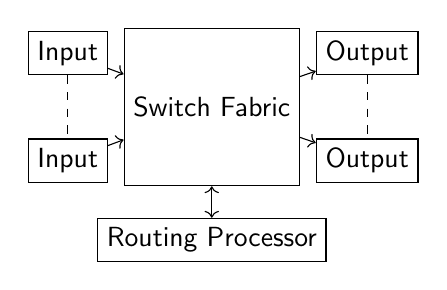
\begin{tikzpicture}[
        node distance=4cm,
        stage/.style={},
        component/.style={
          draw,
          rectangle,
          minimum width=1cm,
          minimum height=0.5cm,
          align=center
        },
        fabric/.style={
          draw,
          rectangle,
          minimum width=1cm,
          minimum height=2cm,
          align=center
        },
        arrow/.style={-Stealth, thick},
        data/.style={midway, above, font=\small}
      ]

      % Main components
      \node[component] (processor) at (0,0) {Routing Processor};

      \node[fabric, above=0.4cm of processor] (fabric) {Switch Fabric};

      % Input interfaces (left side)
      \node[component, above left=0.4cm and 0.2cm of fabric.west] (input1) {Input};
      \node[component, below left=0.4cm and 0.2cm of fabric.west] (input2) {Input};

      % Output interfaces (right side)
      \node[component, above right=0.4cm and 0.2cm of fabric.east] (output1) {Output};
      \node[component, below right=0.4cm and 0.2cm of fabric.east] (output2) {Output};

      % Connections from inputs to fabric
      \draw[->] (input1) -- (fabric);
      \draw[->] (input2) -- (fabric);
      \draw[dashed] (input1) -- (input2);

      % Connections from fabric to outputs
      \draw[->] (fabric) -- (output1);
      \draw[->] (fabric) -- (output2);
      \draw[dashed] (output1) -- (output2);

      \draw[<->] (fabric) -- (processor);

    \end{tikzpicture}
  \end{center}

  \subsubsection{Routing Processor}

  \begin{itemize}
    \item Performs control-plane functions
    \item Executes routing protocols, maintaining routing tables, and computes forwarding table for the router
  \end{itemize}

  \subsubsection{Switch Fabric}

  \begin{itemize}
    \item Responsible for transferring packets between various modules such as NICs, memory blocks, etc.
    \item Forwards packets from input port to output port
  \end{itemize}

  \subsubsection{Router Steps}

  \begin{enumerate}
    \item Packet comes in through input port
    \item Router uses forwarding table to look up output port for the incoming packet
    \item Arriving packet gets forwarded via the switch fabric
    \item Forwarding table is computed/updated by routing processor
    \item Forwarding table is copied by routing processor to the line cards over a separate bus
  \end{enumerate}

  \subsection{IP}

  \begin{itemize}
    \item Identity of the host
    \item Connectionless protocol
    \item Provides internetworking, where routers are used to interconnect heterogeneous networks
    \item Hierarchical addressing, where all hosts in the same network has the same network ID
    \item Used to forward datagrams from one network to another network
    \item Assigned by \textbf{ICANN} to avoid conflicts
    \item Allocated in \textbf{prefixes} which is determined by the network portion
    \item Written by giving the lowest IP address in the block and size of the block
    \item Unreliable service/protocol since it does not guarantee delivery
  \end{itemize}

  \definition{Static}{Permanent (Servers or other important equipment)}

  \definition{Dynamic}{Occasionally changes (Consumers)}

  \definition{Local/Private}{Automatically Generated}

  \definition{Public}{Assigned by \textbf{ISP}}

  \subsubsection{Fragmentation Parameters}

  \begin{center}
    \begin{tabular}{| m{1.2cm} | m{3.6cm} |}
      \hline
      \textbf{Identification}  &
      Carries the packet sequence number
      \\
      \hline
      \textbf{DF Bit}          &
      Do not fragment
      \\
      \hline
      \textbf{MF Bit}          &
      More fragments follow this one
      \\
      \hline
      \textbf{Fragment Offset} &
      Start of the fragment (Multiple of 8)
      \\
      \hline
    \end{tabular}
  \end{center}

  \subsubsection{IPv4}

  \begin{itemize}
    \item 4 byte (32 bit) address and written as four octets/each byte (Each byte can go from 0-255)
    \item Faces address exhaustion, which means that there are not enough address in IPv4
    \item Requires a subnet mask as a result, which is a 32 bit sequence with a sequence of 1s followed by a block of 0s
    \item Resulted in the development of \textbf{NAT} and \textbf{IPv6} due to limited storage
  \end{itemize}

  \definition{NAT}{A process that translates \textbf{private IP} addresses in a local network to a \textbf{public IP}, which enables multiple devices within a private network to share the same public IP address.}

  \definition{Subnet Mask}{A logical subdivision of an IP network that is 32 bits (4 bytes). Dependent on the first byte of the IPv4 address. 255 is for the network and 0 is for the host.}

  \vspace{0.2cm}

  \begin{multicols}{2}
    \begin{center}
      \begin{tabular}{| m{0.5cm} | m{0.6cm} | m{1cm} |}
        \hline
        \textbf{Class A} & 1-126   & 255.0.0.0     \\
        \hline
        \textbf{Class B} & 128-191 & 255.255.0.0   \\
        \hline
        \textbf{Class C} & 192-223 & 255.255.255.0 \\
        \hline
      \end{tabular}
    \end{center}

    \textbf{Note: 127 is a loopback. It is reserved for localhost}

    \columnbreak

    e.g. IPv4 address: 128.112.123.80

    \begin{itemize}
      \item Subnet Mask Class: B
      \item Network: 128.112
      \item Host: 123.80
    \end{itemize}
  \end{multicols}

  \vspace{0.2cm}

  \subsubsection{IPv6}

  \definition{Unicast}{Identifies a single interface.}

  \definition{Anycast}{Identifies a set of interfaces in such a way that a pack sent to an anycast address is delivered to the closest member of the set.}

  \definition{Multicast}{Identifies a group of interfaces in such a way that a packet sent to a multicast address is delivered to all the interfaces in the group}

  \begin{itemize}
    \item 16 byte address (128 bits) and written as eight groups of four hexadecimal digits with colons between groups
    \item e.g. 8000:0000:0000:0000:0134:AF12:1112:EF12
    \item Can be optimized, where leading 0s can be omitted (0134 → 134) and one or more groups of 0s can be removed with ::
    \item 8000:0000:0000:0000:0134:AF12:1112:EF12 → 8000::134:AF12:1112:EF12
    \item IPv4 → IPv6 by just adding :: (192.33.21.46 → ::192.33.21.46)
    \item No fragmentation fields and no header checksum
    \item There are no broadcast address since multicast addresses took over
  \end{itemize}

  \begin{center}
    \begin{tabular}{| m{2cm} | m{2.8cm} |}
      \hline
      \textbf{Extension Header (In Order)} & \textbf{Description}                       \\
      \hline
      Hop-by-hop options                   & Miscellaneous information for routers      \\
      \hline
      Destination options                  & Additional information for the destination \\
      \hline
      Routing                              & Loose list of routers to visit             \\
      \hline
      Fragmentation                        & Management of datagram fragments           \\
      \hline
      Authentication                       & Verification of the sender's identity      \\
      \hline
      Encrypted security payload           & Information about the encrypted contents   \\
      \hline
    \end{tabular}
  \end{center}

  \subsection{Internet Control Protocols}

  \subsubsection{ICMP (Internet Control Message Protocol)}
  \begin{itemize}
    \item Companion to IP that returns error info
    \item Required and used in many ways
    \item If something unexpected occurred, the main even is reported to the \textbf{sender} by the ICMP
  \end{itemize}

  \begin{center}
    \begin{tabular}{| m{2.4cm} | m{2.4cm} |}
      \hline
      \textbf{Message Type}             & \textbf{Description}               \\
      \hline
      Destination unreachable           & Packet could not be delivered      \\
      \hline
      Time exceeded                     & Time to live field hit 0           \\
      \hline
      Source quench                     & Choke packet                       \\
      \hline
      Redirect                          & Teach a router about geography     \\
      \hline
      Echo and Echo reply               & Check if a machine is alive        \\
      \hline
      Timestamp request/reply           & Same as Echo, but with a timestamp \\
      \hline
      Router advertisement/solicitation & Find a nearby router               \\
      \hline
    \end{tabular}
  \end{center}

  \subsubsection{ARP (Address Resolution Protocol)}
  \begin{itemize}
    \item Finds Ethernet address of a local IP address
    \item Provides a mechanism to translate IP address to link-layer addresses
    \item Host queries an address and the owner replies
    \item Resolves the hardware address, where the request ARP broadcasts the request message and the target ARP responds with the target hardware address
  \end{itemize}

  Suppose that \textbf{A} wants to send a datagram to \textbf{B}, where \textbf{B's MAC address} is not in \textbf{A's ARP table}.
  \begin{center}
    \begin{tabular}{| m{2.4cm} | m{2.4cm} |}
      \hline
      \textbf{Same LAN} & \textbf{Different LAN}                                                            \\
      \hline
      \begin{enumerate}
        \item \textbf{A} broadcasts its ARP query packet, containing \textbf{B}'s IP address with a destination MAC address = FF-FF-FF-FF-FF-FF
        \item \textbf{B} receives the ARP packet, replies to \textbf{A} with its MAC address and the frame is sent to \textbf{A}'s MAC address (unicast)
        \item \textbf{A} caches IP-to-MAC address pair in its ARP table until information times out unless refreshed (plug-and-play)
      \end{enumerate}
      &
      \bul{Data sent must use an intermediate \textbf{R}}
      \begin{enumerate}
        \item Focus on addressing at IP (datagram) and MAC layer (frame)
        \item Assume \textbf{A} knows \textbf{B}'s IP address
        \item Assume \textbf{A} knows IP address of the first hop router, which is configured with the gateway
        \item Assume \textbf{A} knows \textbf{R}'s MAC address by using the ARP
      \end{enumerate} \\
      \hline
    \end{tabular}
  \end{center}

  \subsubsection{DHCP (Dynamic Host Configuration Protocol)}

  \begin{itemize}
    \item Assigns a local IP address to host (either get it through hard coded by the system admin in a file or dynamically get the address from a server)
    \item Gets host started by automatically configuring it
    \item Host sends request to server, which grants a lease
    \item Can return the allocated IP address on a subnet along with the address of the first-hop router for the client (default gateway), name and IP address of the DNS server, and a network mask, which indicates network and host portion of the address
    \item Technically also part of level 7 since it manipulates layer 2 based on responses arrive through level 7
    \item Four step process
  \end{itemize}

  \begin{center}
    \begin{tabular}{| m{1.2cm} | m{3.6cm} |}
      \hline
      \textbf{DHCPDISCOVER} & Host broadcasts the message (OPTIONAL).                                                                \\
      \hline
      \textbf{DHCPOFFER}    & DHCP server responds with message (OPTIONAL).                                                          \\
      \hline
      \textbf{DHCPREQUEST}  & Host requests IP address and receives a message.                                                       \\
      \hline
      \textbf{DHCPACK}      & Sent by servers to acknowledge the DHCPREQUEST and to finalize the lease of an IP address to a client. \\
      \hline
    \end{tabular}
  \end{center}

  \subsection{Network Topologies}

  \begin{center}
    \begin{tabular}{| m{0.5cm} | m{4.3cm} |}
      \hline
      \textbf{Bus}  &
      \bul{All nodes are connected to single bidirectional communication line/cable called the trunk (backbone or segment)}
      \bul{Simple and low cost}
      \bul{One computer can send messages at a times}
      \bul{Passive topology - computers only listen for, not regenerate data}     \\
      \hline
      \textbf{Star} &
      \bul{Centers on one node where all the others are connected and through which messages are sent}
      \bul{More cabling, thus higher costs}
      \bul{If the hub (switch) is down, no communication}
      \bul{Depending on hub, multiple devices can send messages at the same time} \\
      \hline
      \textbf{Ring} &
      \bul{All nodes connected in a loop/ring and unidirectional}
      \bul{Each computer serves as a repeater}
      \bul{Typical way to send data by token passing}
      \bul{Expensive and difficult to add computers}
      \bul{If one computer fails, whole network fails}                            \\
      \hline
    \end{tabular}
  \end{center}

  \subsection{Design Issues}

  \begin{itemize}
    \item Store-and-Forward Packet Switching (Each router needs to store the entire packet before it can forward it to the next hop)
    \item Services to Transport Layer (Provides service its immediate upper layer, namely transport layer, through the network transport layer interface)
    \item Providing Connection Oriented Service
    \item Providing Connectionless Service
  \end{itemize}

  \subsection{Internetworking}

  \begin{itemize}
    \item Joins multiple, different networks into a single larger network
    \item Networks differ by services, packet size, reliability, security, addressing. etc.
    \item Connect by providing a common layer to hide differences (common IP layer since IP provides a universal packet format that all routers recognize)
  \end{itemize}

  \section{Data Link Layer}

  \subtitle{Frames}{Hop-to-Hop Delivery}

  \subsection{Definitions}

  \definition{Carrier Sense Multiple Access / Collision Detection (CSMA/CD)}{A network access method primarily used in wired Ethernet networks, where multiple devices share a single transmission medium.}

  \definition{Cyclic Redundancy Check (CRC)}{An error detecting piece of code used to verify integrity by generating a checksum.}

  \definition{Link Layer Address}{Name that can also be called a \textbf{LAN} address, a physical address, or a \textbf{MAC} address}

  \definition{Switch Table}{A table that has the information on what interface to use to reach a specific device.}

  \subsection{Services}

  \subsubsection{Framing}
  \begin{itemize}
    \item All layer protocols encapsulate each network-layer datagram within a link-layer frame before transmission over the link
    \item Frame consists of a data field, in which the network-layer datagram is inserted, and a number of header fields
    \item Structure specified by link layer protocol
  \end{itemize}

  \subsubsection{Link Access}

  \begin{itemize}
    \item A medium access control (MAC) protocol specifies the rules by which a frame is transmitted onto the link
    \item e.g. point-to-point links that have a single sender at one end of the link and a single receiver at the other end of the link, the MAC protocol is simple, the sender can send a frame
      whenever the link is idle
  \end{itemize}

  \subsubsection{Reliable Delivery}

  Note: The link-layer reliable delivery can be considered an unnecessary overhead for low bit-error links, including fiber coax, and many twisted-pair copper link

  \begin{itemize}
    \item When a link-layer protocol provides reliable delivery service, it guarantees to move each network-layer datagram across the link without error
    \item Similar to a transport-layer reliable delivery service, a link-layer reliable delivery service can be achieved with acknowledgements and retransmissions
    \item Similar to a transport-layer reliable delivery service, a link-layer reliable delivery service can be achieved with acknowledgements and retransmissions
    \item Many wired link-layer protocols do not provide a reliable delivery service
  \end{itemize}

  \subsubsection{Error Detection and Correction}

  Error correction is similar to error detection, except that a receiver not only detects when bit errors have occurred in the frame but also determines exactly where in the frame the errors have occurred (also corrects these errors)

  \begin{itemize}
    \item Link-layer hardware in a receiving node can incorrectly decide that a bit in a frame is zero when it was transmitted as a one, and vice versa
    \item No need to forward a datagram that has an error, many link-layer protocols provide a mechanism to detect such bit errors
    \item Done by having the transmitting node include error-detection bits in the frame, and having the receiving node perform an error check
    \item Usually more sophisticated and is implemented in hardware
  \end{itemize}

  \subsection{Devices}

  \begin{center}
    \begin{tabular}{| m{0.7cm} | m{4.1cm} |}
      \hline
      \textbf{Switches}                       &
      \bul{Full-duplex (Switching can be done without collisions)}
      \bul{Replaces hubs}
      \bul{Connects different devices on the same network and only intended nodes receives transmissions}
      \bul{Uses a switch table and updates it with incoming frames (learns location of sender and LAN segment)}
      \bul{Fast and secure}
      \bul{Stores and forwards Ethernet frames}
      \bul{Examine incoming frame's MAC address and selectively forward to one or more outgoing links when forwarded on segment}
      \bul{Uses CSMA/CD to access segment}
      \bul{Do not need to be configured (plug-and-play, self-learning)}
      \bul{Hosts unaware of the presence of switches}
      \bul{Hosts have dedicated, direct connection to switches}
      \bul{Buffer packets}
      \\
      \hline
      \textbf{Network Interface Cards (NICs)} &
      \bul{Level 1 (Physical item) \& 2 (Deals with MAC addressing)}
      \bul{A network adaptor that connects node to the media}
      \bul{Unique MAC address}
      \\
      \hline
    \end{tabular}
  \end{center}

  \subsection{Sub-Layers}

  \begin{center}
    \begin{tabular}{| m{0.7cm} | m{4.1cm} |}
      \hline
      \textbf{Media Access Control (MAC)} &
      \bul{Gives access to the NIC}
      \bul{Controls access to through media through CSMA/CD and token passing}
      \\
      \hline
      \textbf{Logical Link Control (LLC)} &
      \bul{Manages data link interface}
      \bul{Responsible for error detection and ensuring data integrity}
      \bul{Detects transmission errors using CRC and will request any resends}
      \\
      \hline
    \end{tabular}
  \end{center}

  \subsection{Implementation}

  \begin{itemize}
    \item Combination of hardware and software, the place in the protocol stack where software meets hardware
    \item Implemented in a network adaptor, also sometimes known as a \textbf{NIC}
    \item Network adaptor is the link-layer controller (Usually a single, special-purpose chip that implements many of the link-layer services (framing, link access, error detection, and so on))
    \item Much of a link-layer controller’s functionality is
      implemented in hardware
  \end{itemize}

  \begin{center}
    \begin{tabular}{| m{1cm} | m{3.8cm} |}
      \hline
      \textbf{Source}      &
      The controller does the following: \par
      \begin{enumerate}
        \item Takes a datagram that has been created and stored in host memory by the higher layers of the protocol stack
        \item Encapsulates the datagram in a link-layer frame (Filling in the frame's various fields)
        \item Transmits the frame into the communication link, following the
          link-access protocol
      \end{enumerate}
      \\
      \hline
      \textbf{Destination} &
      The controller does the following:
      \begin{enumerate}
        \item Receives the entire frame
        \item Extracts the network-layer datagram
      \end{enumerate}
      \bul{If the link layer performs error detection, then it is the sending controller that sets the error-detection bits in the frame header, and it is the receiving controller that performs error detection}
      \\
      \hline
    \end{tabular}
  \end{center}

  \subsection{MAC Address}

  \begin{itemize}
    \item 48-bit (6 bytes/6 paired hexadecimal values) unique identifier administered by IEEE
    \item $2^{48}$ possible addresses
    \item Used to identify a device on a network (no two adaptors have the same address)
    \item Flat structure (MAC address resembles a person's social security number)
    \item Were designed to be permanent, but now possible to change through software
    \item IEEE manages the MAC addresses
    \item Manufacturers buys portions of MAC address space consisting of $2^{24}$ addresses for a nominal fee
    \item IEEE allocates the chunk of $2^{24}$ addresses by fixing the first 24 bits of a MAC address and letting the company create unique combinations of the last 24 bits for each adaptor
    \item Used for level 2 addressing
    \item Burned onto NIC ROM and sometimes software settable
    \item e.g. 1A-2B-3C-4D-5E-6F

    \item Portable, unlike IP addresses
  \end{itemize}

  \subsection{Ethernet}

  \begin{itemize}
    \item Level 2 and 1 item
    \item Dominant wired LAN technology that is cheap and simple
    \item 10 Mbps - 400 Gbps
    \item Single chip, multiple speeds
    \item Used to use \textbf{bus} topology back in the mid 90s, now using \textbf{star} topology
    \item Connectionless (No handshaking between sending and receiving NICs)
    \item Unreliable (Receiving NICs doesn't send ACK or NAK to sending NIC)
    \item Ethernet's MAC protocol: Unslotted CSMA/CD with binary backoff
  \end{itemize}

  \subsubsection{Parts of the Ethernet Packet and Frame (In order)}

  \begin{center}
    \begin{tabular}{| m{1.3cm} | m{0.4cm} | m{3.1cm}|}
      \hline
      \textbf{Part}                     & \textbf{Bytes} & \textbf{Information} \\
      \hline
      \textbf{Preamble}                 & 7              &
      \bul{Used to synchronize receiver}
      \bul{7 bytes of 10101010}
      \bul{Not part of the frame}
      \\
      \hline
      \textbf{Starting Frame Delimiter} & 1              &
      \bul{Indicates beginning of Ethernet frame}
      \bul{10101011}
      \bul{Not part of the frame}
      \\
      \hline
      \textbf{MAC Destination}          & 6              &
      \bul{Address of device the packet is intended for}
      \bul{Adaptor passes data in frame to network layer if frame has matching destination address; otherwise thrown out}
      \\
      \hline
      \textbf{MAC Source}               & 6              &
      \bul{Address of device the packet originated for}
      \\
      \hline
      \textbf{Payload (Data)}           & 42-1500        &
      \bul{Data to be sent}
      \\
      \hline
      \textbf{EtherType (Type)}         & 2              &
      \bul{Used to indicate which protocol is encapsulated in the payload of the frame and used for receiving}
      \bul{Mostly IP but others possible like AppleTalk or Novell IPX}
      \bul{Used to demultiplex at receiver}
      \\
      \hline
      \textbf{CRC}                      & 4              &
      \bul{Checks redundancy at receiver}
      \bul{Thrown out if error detected}
      \\
      \hline
    \end{tabular}
  \end{center}

  \subsubsection{Enterprise Access Networks}

  \begin{itemize}
    \item Typically used in companies, universities, or any large organization
    \item Various transmission rates, ranging from 10Mbps to 10Gbps
    \item End systems typically connect to Ethernet switch
  \end{itemize}

  \section{Physical Layer}

  \subtitle{Bits}{Bit-to-Bit Delivery}

  \subsection{Definitions}

  \definition{Bandwidth (Electrical Engineering)}{A measure of the
  width of a frequency range. Measured with \textbf{hz}.}

  \definition{Bandwidth (Computer Scientists)}{Rate of data transfer.
  Measured in \textbf{bps}}

  \definition{Digital Modulation}{The process of converting data bits
  into signals.}

  \definition{Frequency (f)}{\# of oscillations per second measured using \textbf{hz}}

  \definition{Harmonic}{A sinusoidal wave with a frequency that is a positive integer multiple of a fundamental frequency of a periodic signal.}

  \definition{Modulation}{Process of varying one or more properties of a periodic waveform (the carrier signal) to encode information onto it.}

  \definition{Period (T)}{Time between two consecutive max or min. $T = 1/f$}

  \definition{STP}{Type of copper cable that consists of a pair of wires twisted together. Has an additional shield layer to reduce interference, but harder to install and more expensive.}

  \definition{UTP}{Type of copper cable that consists of a pair of wires twisted together. Does not have an additional shield layer.}

  \definition{Wavelength ($\lambda$)}{Distance between two max or min. $\lambda = c/f$ in a vacuum.}

  \subsection{Devices}

  \begin{center}
    \begin{tabular}{| m{0.7cm} | m{4.1cm} |}
      \hline
      \textbf{Hub}      &
      \bul{Center of star network}
      \bul{All nodes receive transmitted packets}
      \bul{Slow and insecure}                                              \\
      \hline
      \textbf{Repeater} &
      \bul{Repeats signal since signals lose intensity due to energy loss} \\
      \hline
    \end{tabular}
  \end{center}

  \subsection{General Information}

  \begin{itemize}
    \item Foundation where other layers are built on
    \item Determines \textbf{throughput}, \textbf{latency}, \textbf{error rate}
    \item Modulation needed to convert analog to digital
  \end{itemize}

  \subsection{Fourier Analysis}

  $$g(t) = \frac{c}{2} + \sum_{n = 1}^{\infty}a_n\sin(2\pi \text{nft}) + \sum_{n = 1}^{\infty}b_n\cos(2\pi \text{nft})$$

  \begin{itemize}
    \item Time varying signal can be represented harmonics or
      infinite number of sines and cosines
    \item $a_n$ and $b_n$ are the sine and cosine amplitudes of the
      nth harmonic (terms) and c is a constant
  \end{itemize}

  \begin{multicols*}{2}
    \subsection{Bandwidth-Limited Signals}

    \begin{itemize}
      \item Having less bandwidth = losing some harmonics
      \item Degrades the received signal
    \end{itemize}

    \subsection{Media Properties}
    \begin{itemize}
      \item Bandwidth
      \item Delay
      \item Cost
      \item Ease of installation
      \item Maintenance
    \end{itemize}

    \columnbreak

    \subsection{Guided Media}
    \begin{itemize}
      \item Copper Wire (Twisted pairs, Coaxial Cable, Power lines)
      \item Fiber Optics (Single-mode, Multi-mode)
    \end{itemize}

    \subsection{Unguided Media}
    \begin{itemize}
      \item Terrestrial wireless
      \item Satellite
      \item Lasers through the air
    \end{itemize}
  \end{multicols*}

  \subsection{Wires}

  \subsubsection{Link Terminology}
  \begin{center}
    \begin{tabular}{| m{1cm} | m{3.8cm} |}
      \hline
      \textbf{Full-duplex} &
      \bul{Bidirectional simultaneous transmission}
      \bul{e.g. Use different twisted pairs for each direction} \\
      \hline
      \textbf{Half-duplex} &
      \bul{Bidirectional but not simultaneous transmission}
      \bul{e.g. Senders taking turns}                           \\
      \hline
      \textbf{Simplex}     &
      \bul{Only one fixed direction at all times}
      \bul{Not common}                                          \\
      \hline
    \end{tabular}
  \end{center}

  \subsubsection{Twisted Pair}

  \begin{itemize}
    \item Two insulated copper wires
    \item Used in LANs and telephone lines
    \item Twists reduce radiated signal (interference)
    \item Signal carried as the difference in voltage between two wires
  \end{itemize}

  \begin{center}
    \begin{tabular}{| m{1.3cm} | m{3.5cm} |}
      \hline
      \textbf{Category 5 (CAT5)}   &
      \bul{Half-duplex and \textbf{UTP}}
      \bul{Has 4 twisted wire pairs}
      \bul{100Mbps Fast Ethernet uses two pairs, one for each direction}
      \bul{1 Gbps Ethernet uses all four pairs in both directions simultaneously}                                   \\
      \hline
      \textbf{Category 5e (CAT5e)} &
      \bul{Enhanced version of CAT5}
      \bul{Significantly improved performance and network capabilities (1000Mbps Gigabit Ethernet and Full-duplex)} \\
      \hline
      \textbf{Category 6 (CAT6)}   &
      \bul{Full-duplex and \textbf{UTP}}
      \bul{Compatible with CAT5}
      \bul{10 Gbps, thus faster}
      \bul{More stringent (strict) specifications for crosstalk and system noise, up to 100 m.}                     \\
      \hline
      \textbf{Category 7 (CAT7)}   &
      \bul{Full-duplex and \textbf{STP}}
      \bul{Backwards compatible}
      \bul{Not recognized by TIA/EIA (Not as used)}                                                                 \\
      \hline
    \end{tabular}
  \end{center}

  \subsubsection{Coaxial}

  \begin{itemize}
    \item \textbf{Half-duplex}, but can enable full-duplex like behavior
    \item Two concentric copper conductors
    \item Common but more expensive than twisted pair
    \item Better shielding, more bandwidth for longer distances, and higher rates than twisted pair
    \item Used for video and TV since it needs larger bandwidth
    \item Replaced by fiber optic
  \end{itemize}

  \definition{50-ohm}{Used for digital transmission.}

  \definition{75-ohm}{Used for analog transmission, but now used for both digital and analog.}

  \subsubsection{Internet Over Cable}

  \begin{itemize}
    \item Reuses cable television plant
    \item Data sent on the shared cable tree from the head-end, not on a dedicated line per subscriber, unlike \textbf{DSL}
    \item Uses \textbf{FDM}
  \end{itemize}

  \subsection{Power Lines}

  \begin{itemize}
    \item Household electrical wiring
    \item 50-60Hz, too low for data
  \end{itemize}

  \subsection{Fiber Optics}

  \begin{itemize}
    \item Glass fiber carrying light pulses
    \item Pulse of light is 1 bit whereas no light pulse indicates 0
    \item Low error rate, thus more sparsely placed repeaters (light is immune to electromagnetic noises)
    \item Common for high data rates and long distances
    \item Three components: Light source, transmission media, and detector (generates pulse when light falls on it)
  \end{itemize}

  \begin{center}
    \begin{tabular}{| m{2.4cm} |  m{2.4cm}|}
      \hline
      \textbf{Single-Mode} & \textbf{Multi-Mode}              \\
      \hline
      \bul{Narrow core (10 \text{\textmu{}}m)}
      \bul{Light can not bounce}
      \bul{Used for lasers of long distances}
      &
      \bul{50 \text{\textmu{}}m core diameter}
      \bul{Light can bounce}
      \bul{Used for LEDs for cheaper, shorter distance links} \\
      \hline
    \end{tabular}
  \end{center}

  \subsubsection{FTTH}

  \begin{itemize}
    \item Relies on the deployment of fiber optic cables to provide higher data rates to customers
    \item One wavelength for many houses
    \item Fiber is passive, so no amplifiers are needed
    \item Up to 100Mbps
  \end{itemize}

  \subsection{Wireless Transmission}

  \begin{center}
    \begin{tabular}{| m{2.4cm} |  m{2.4cm}|}
      \hline
      \textbf{Pros} & \textbf{Cons}                               \\
      \hline
      \bul{Easy and inexpensive to deploy}
      \bul{Naturally supports mobility and broadcast}
      &
      \bul{Transmissions interfere and must be managed}
      \bul{Signal strengths vary, resulting in varied data rates} \\
      \hline
    \end{tabular}
  \end{center}

  \subsection{Electromagnetic Spectrum}

  \begin{itemize}
    \item Signal carried in electromagnetic spectrum
    \item Travels at a speed of $c = 3 \times 10^8 \text{m/ sec}$
    \item Different bands like radio, microwave, infrared, UV, X-Ray, Gamma Ray
  \end{itemize}

  \begin{multicols}{3}

    \subsection{WAN}

    \begin{itemize}
      \item Shared wireless access network connects end system to router via base station (access point \textbf{AP})
    \end{itemize}

    \vspace*{\fill}

    \columnbreak

    \subsubsection{WLAN}

    \begin{itemize}
      \item Within building, around 100 ft
      \item IEEE 802.11 g/n/ac (Wi-Fi): 54/300/1000 Mbps transmission rate
    \end{itemize}

    \vspace*{\fill}

    \columnbreak

    \subsubsection{WWAN}

    \begin{itemize}
      \item Cellular data (2G, 3G, 4G, LTE, 5G)
      \item Between 1 and 100 Mbps and more
    \end{itemize}
  \end{multicols}

  \subsection{Baseband Transmission}

  \begin{itemize}
    \item 4B/5B coding scheme
    \item Signal occupies frequencies from zero to a maximum
    \item Common for wires
    \item Introduced to limit the number of consecutive 0s or 1s
    \item Every 4 bits is mapped into 5 bit pattern with a \textbf{fixed} translation table (e.g. 0000 → 11110)
  \end{itemize}

  \begin{multicols}{2}
    \subsubsection{Non-Return-to-Zero (NRZ)}

    \begin{itemize}
      \item Use a positive voltage to represent 1, negative voltage to represent 0
      \item More levels of voltages means that the symbol carries more bits
    \end{itemize}

    \columnbreak

    \subsubsection{Non-Return-to-Zero Inverted (NRZI)}

    \begin{itemize}
      \item Same as NRZ, but code the one as transition and zero as no transition (or opposite way)
    \end{itemize}
  \end{multicols}

  \subsubsection{Manchester Encoding}

  \begin{itemize}
    \item Mixes clock signal with data signal by using XOR
    \item When the clock is XORed with 0, it makes a low-to-high transition (logical 0)
    \item When the clock is XORed with 1, it makes a high-to-low transition (logical 1)
  \end{itemize}

  \subsection{Passband Transmission}

  \begin{itemize}
    \item Schemes that regulate the amplitude, phase, or frequency of the carrier signal to convey bits
    \item Occupies a band of frequencies around the frequency of the carrier signal that does \textbf{not} start at 0
    \item Not practical for wireless channels to send very low frequencies since size of the antenna ($\lambda/4$) would be large ($\lambda = c/f$)
    \item Common for wireless and optical channels
    \item Governed by regulated body
    \item Digital modulation is accomplished by modulating the carrier signal that sits in the passband
  \end{itemize}

  \subsubsection{Modulation Methods}

  \begin{center}
    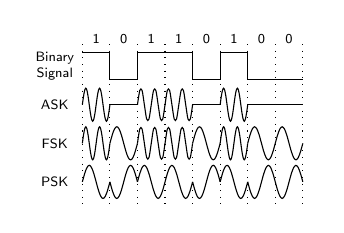
\begin{tikzpicture}[
        block/.style={draw, rectangle, minimum height=1.5em, minimum width=3em, font=\scriptsize},
        >=Stealth,
        font=\scriptsize,
        scale=0.7,
        every node/.style={transform shape}
      ]

      % Digital data
      \node [yshift=0cm, text width = 0.75cm, align = center] (BS) {Binary Signal};
      \node [yshift=-0.7cm, text width = 0.75cm, align = center] (ASK) {ASK};
      \node [yshift=-1.4cm, text width = 0.75cm, align = center] (FSK) {FSK};
      \node [yshift=-2.1cm, text width = 0.75cm, align = center] (PSK) {PSK};

      \node [yshift=0.5cm, xshift=0.75cm, text width = 0.75cm, align = center] {1};
      \node [yshift=0.5cm, xshift=1.25cm, text width = 0.75cm, align = center] {0};
      \node [yshift=0.5cm, xshift=1.75cm, text width = 0.75cm, align = center] {1};
      \node [yshift=0.5cm, xshift=2.25cm, text width = 0.75cm, align = center] {1};
      \node [yshift=0.5cm, xshift=2.75cm, text width = 0.75cm, align = center] {0};
      \node [yshift=0.5cm, xshift=3.25cm, text width = 0.75cm, align = center] {1};
      \node [yshift=0.5cm, xshift=3.75cm, text width = 0.75cm, align = center] {0};
      \node [yshift=0.5cm, xshift=4.25cm, text width = 0.75cm, align = center] {0};

      \draw[dotted] (0.5, 0.4) -- (0.5, -2.5);
      \draw[dotted] (1, 0.4) -- (1, -2.5);
      \draw[dotted] (1.5, 0.4) -- (1.5, -2.5);
      \draw[dotted] (2, 0.4) -- (2, -2.5);
      \draw[dotted] (2.5, 0.4) -- (2.5, -2.5);
      \draw[dotted] (3, 0.4) -- (3, -2.5);
      \draw[dotted] (3.5, 0.4) -- (3.5, -2.5);
      \draw[dotted] (4, 0.4) -- (4, -2.5);
      \draw[dotted] (4.5, 0.4) -- (4.5, -2.5);

      % Modulation process
      \draw (0.5,0.25) -- (1,0.25) -- (1,-0.25) -- (1.5,-0.25) -- (1.5,0.25) -- (2,0.25) -- (2.5,0.25) -- (2.5,-0.25) -- (3,-0.25) -- (3,0.25) -- (3.5,0.25) -- (3.5,-0.25) -- (4.5,-0.25);

      % Modulated signal (ASK example)
      \draw[domain=0:0.5,smooth,variable=\x] plot ({\x + 0.5},{-0.7+0.3*sin(4 * pi / 0.5 *\x r)});

      \draw[domain=0.5:1,smooth,variable=\x] plot ({\x + 0.5},{-0.7});

      \draw[domain=1:2,smooth,variable=\x] plot ({\x + 0.5},{-0.7+0.3*sin(4 * pi / 0.5 *\x r)});

      \draw[domain=2:2.5,smooth,variable=\x] plot ({\x + 0.5},{-0.7});

      \draw[domain=2.5:3,smooth,variable=\x] plot ({\x + 0.5},{-0.7+0.3*sin(4 * pi / 0.5 *\x r)});

      \draw[domain=3:4,smooth,variable=\x] plot ({\x + 0.5},{-0.7});

      % Modulated signal (FSK example)
      \draw[domain=0:0.5,smooth,variable=\x] plot ({\x + 0.5},{-1.4+0.3*sin(4 * pi / 0.5 *\x r)});

      \draw[domain=0.5:1,smooth,variable=\x] plot ({\x + 0.5},{-1.4+0.3*sin(2 * pi / 0.5 *\x r)});

      \draw[domain=1:2,smooth,variable=\x] plot ({\x + 0.5},{-1.4+0.3*sin(4 * pi / 0.5 *\x r)});

      \draw[domain=2:2.5,smooth,variable=\x] plot ({\x + 0.5},{-1.4+0.3*sin(2 * pi / 0.5 *\x r)});

      \draw[domain=2.5:3,smooth,variable=\x] plot ({\x + 0.5},{-1.4+0.3*sin(4 * pi / 0.5 *\x r)});

      \draw[domain=3:4,smooth,variable=\x] plot ({\x + 0.5},{-1.4+0.3*sin(2 * pi / 0.5 *\x r)});

      % Modulated signal (PSK example)
      \draw[domain=0:0.5,smooth,variable=\x] plot ({\x + 0.5},{-2.1+0.3*sin(2 * pi / 0.5 *\x r)});

      \draw[domain=0.5:1,smooth,variable=\x] plot ({\x + 0.5},{-2.1-0.3*sin(2 * pi / 0.5 *\x r)});

      \draw[domain=1:2,smooth,variable=\x] plot ({\x + 0.5},{-2.1+0.3*sin(2 * pi / 0.5 *\x r)});

      \draw[domain=2:2.5,smooth,variable=\x] plot ({\x + 0.5},{-2.1-0.3*sin(2 * pi / 0.5 *\x r)});

      \draw[domain=2.5:3,smooth,variable=\x] plot ({\x + 0.5},{-2.1+0.3*sin(2 * pi / 0.5 *\x r)});

      \draw[domain=3:4,smooth,variable=\x] plot ({\x + 0.5},{-2.1-0.3*sin(2 * pi / 0.5 *\x r)});

    \end{tikzpicture}
  \end{center}

  \begin{center}
    \begin{tabular}{| m{0.3cm} |  m{4.5cm}|}
      \hline
      \textbf{ASK} & Use two different amplitudes to represent 0 and 1.                                                                     \\
      \hline
      \textbf{FSK} & Two or more frequencies are used.                                                                                      \\
      \hline
      \textbf{PSK} & Carrier wave is shifted $\theta$ degrees at each symbol period. If there are two phases, this is called \textbf{BPSK}. \\
      \hline
    \end{tabular}
  \end{center}

  \section{Calculations}

  \subsection{One's Complement}
  Invert all bits (1 → 0 and 0 → 1) ($11010101 \rightarrow 00101010$)

  \subsection{TCP Acknowledgement Number}

  Acknowledgement Number = Sequence Number + Size of Segment

  e.g. 356-byte segment has a sequence number field of 2512. ($356 + 2512 = 2868$ is the Acknowledgement)

  \textbf{Next sequence number would be the acknowledgement number!}

  \subsection{UDP Packet Checksum}

  \begin{enumerate}
    \item Calculate the one's complement sum.
    \item Move the leading bit (most significant value) and add to the end if more than 4 hexadecimal values.
    \item Find the one's complement of the sum.
    \item Convert back to hexadecimal.
  \end{enumerate}

  e.g. 4510, 003C, 1C46, 4501, 4006, B1E6, AC10, 1A63
  \begin{align*}
    \text{SUM}       & = 0x25EF2                            \\
    0x25EF2          & \rightarrow 0x5EF4 (0x5EF2 + 0x0002) \\
    0x5EF4           & \rightarrow 0101111011110100         \\
    0101111011110100 & \rightarrow 1010000100001011         \\
    1010000100001011 & \rightarrow 0xA10B                   \\
  \end{align*}

  \section{Packet Tracer}

  \begin{itemize}
    \item Copper Stright-Through wires for different level (computer to switch)
    \item Copper Cross-Over wires for same level (switch to switch)
    \item Use the Home Router since none of the other routers work
    \item For laptop, add Linksys-WPC300N connector to make wireless (must power off first)
    \item "ping IPv4-ADDRESS-HERE" to check if current device is connected to another device
  \end{itemize}

  \section{Sockets}

  \subsection{Definitions}

  \definition{Sockets (kernel)}{Endpoint of communication.}

  \definition{Sockets (application)}{File descriptor that lets application \textbf{RO} from/to network}

  \subsection{General}

  \begin{itemize}
    \item Consists of a pair of programs: \textbf{client} and \textbf{server}
    \item When programs are executed, a client and a server process are created, and these processes communicate with each other by reading from and writing to sockets
    \item e.g. A client reads a string from its keyboard and sends it to the server, where the server gets the data and converts it to uppercase, sending it back to the client where the client displays it
  \end{itemize}

  \subsection{General Socket Information}

  \begin{multicols*}{2}
    \subsubsection{Address Family}

    \begin{center}
      \begin{tabular}{| m{1cm} | m{1.0cm} |}
        \hline
        \textbf{AF_INET}  & IPv4 \\
        \hline
        \textbf{AF_INET6} & IPv6 \\
        \hline
        \textbf{AF_UNIX}  & Unix \\
        \hline
      \end{tabular}
    \end{center}

    \columnbreak

    \subsubsection{Socket Type}

    \begin{center}
      \begin{tabular}{| m{1.2cm} | m{1.0cm} |}
        \hline
        \textbf{SOCK_STREAM} & TCP \\
        \hline
        \textbf{SOCK_DGRAM}  & UDP \\
        \hline
        \textbf{SOCK_RAW}    & Raw \\
        \hline
      \end{tabular}
    \end{center}
  \end{multicols*}

  \vspace{0.2cm}

  \subsubsection{Functions}

  \begin{center}
    \begin{tabular}{| m{1cm} | m{3.8cm} |}
      \hline
      \textbf{accept()}             & Accepts an incoming connection request, returning a new socket for the connection.
      \\
      \hline
      \textbf{bind()}               & Assigns a local socket address to a socket, allowing the server to listen for connections.
      \\
      \hline
      \textbf{connect()}            & Connects a client socket to a server socket address, establishing a connection.
      \\
      \hline
      \textbf{sendto(), recvfrom()} & Used for sending and receiving data with \textbf{UDP} sockets, where destination and source addresses are specified using socket address structures
      \\
      \hline
    \end{tabular}
  \end{center}

  \begin{center}
    \begin{tabular}{| m{0.5cm} | m{4.3cm} |}
    \end{tabular}
  \end{center}

  \subsection{UDP Socket Programming}

  \begin{center}
    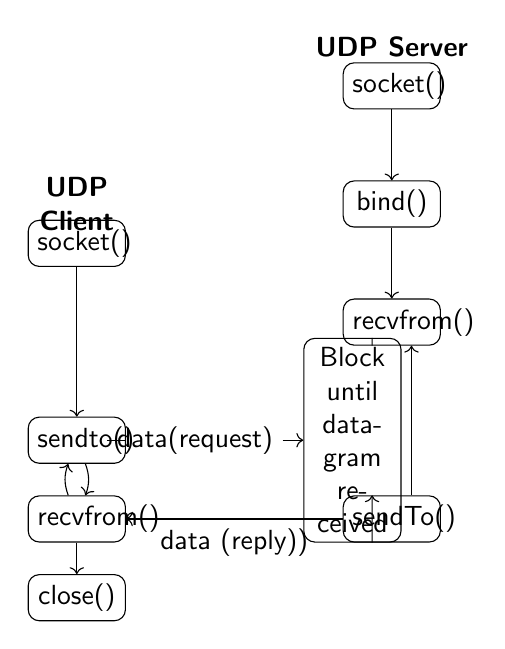
\begin{tikzpicture}[
        node distance=4cm,
        every arrow/.style={thick,>=stealth},
        data/.style={midway, above}
      ]

      % Client steps
      \node[font=\bfseries, align=center, text width = 1cm] (client) at (-2, -0.5) {UDP Client};
      \node[align=center, text width=1cm, draw, rounded corners] (clientSocket) at (-2, -1) {socket()};
      \node[align=center, text width=1cm, draw, rounded corners] (clientSend) at (-2, -3.5) {sendto()};
      \node[align=center, text width=1cm, draw, rounded corners] (clientReceive) at (-2, -4.5) {recvfrom()};
      \node[align=center, text width=1cm, draw, rounded corners] (clientClose) at (-2, -5.5) {close()};

      \draw[->] (clientSocket) -- (clientSend);
      \draw[->] (clientSend) to[bend left=20] (clientReceive);
      \draw[->] (clientReceive) to[bend left=20] (clientSend);
      \draw[->] (clientReceive) -- (clientClose);

      % Server steps
      \node[font=\bfseries, align=center] (server) at (2, 1.5) {UDP Server};
      \node[align=center, text width=1cm, draw, rounded corners] (serverSocket) at (2, 1){socket()};
      \node[align=center, text width=1cm, draw, rounded corners] (serverBind) at (2, -0.5){bind()};
      \node[align=center, text width=1cm, draw, rounded corners] (serverReceive) at (2, -2){recvfrom()};
      \node[align=center, text width=1cm, draw, rounded corners] (serverSend) at (2, -4.5){sendTo()};

      % Arrows
      \draw[->] (serverSocket) -- (serverBind);
      \draw[->] (serverBind) -- (serverReceive);

      \node[align=center, text width=1cm, draw, rounded corners] (block) at (1.5, -3.5) {Block until datagram received};

      \draw[->] ([xshift=0.25cm]serverSend.north) -- ([xshift=0.25cm]serverReceive.south);

      \node[align=center] (datareq) at (-0.5, -3.5){data(request)};
      \draw[->] (clientSend) -- (datareq) -- (block);
      \draw[-] ([xshift=-0.25cm]serverReceive.south) -- ([xshift=0.25cm]block.north);
      \draw[->] ([xshift=0.25cm]block.south) -- ([xshift=-0.25cm]serverSend.north);

    \draw[->] (serverSend) -- node[sloped, below] {data (reply))} ([yshift=-4mm]clientReceive);
  \end{tikzpicture}

\end{center}

\textbf{Use for speed and when some data loss is acceptable.}

\begin{itemize}
  \item Provides unreliable transfer of datagrams between client and server
  \item No "connection" between client and server since no handshaking
  \item Sender program explicitly attaches IP destination address and port \# to each packet.
  \item Transmitted data may be lost or out of order when received
\end{itemize}

\subsection{TCP Socket Programming}

\begin{center}
  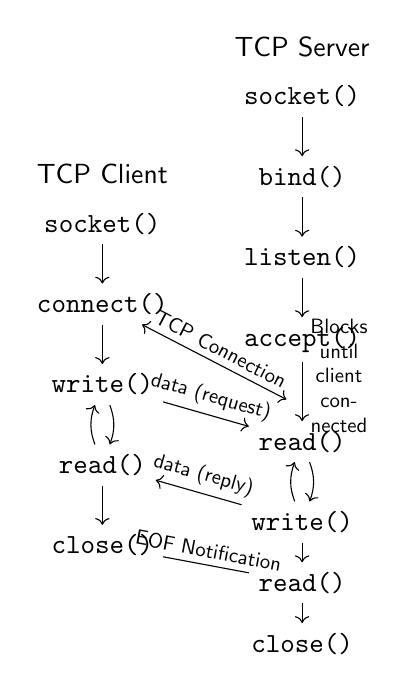
\begin{tikzpicture}[
      node distance=4cm,
      stage/.style={},
      arrow/.style={-Stealth, thick},
      data/.style={midway, above, font=\small}
    ]

    % Nodes
    \node[stage] (client) {TCP Client};
    \node[stage, above right=1.125cm and 0.6cm of client] (server) {TCP Server};

    % Client steps
    \node[below=0.125cm of client] (clientSocket) {\texttt{socket()}};
    \node[below=0.5cm of clientSocket] (clientConnect) {\texttt{connect()}};
    \node[below=0.5cm of clientConnect] (clientWrite) {\texttt{write()}};
    \node[below=0.5cm of clientWrite] (clientRead) {\texttt{read()}};
    \node[below=0.5cm of clientRead] (clientClose) {\texttt{close()}};

    \draw[->] (clientSocket) -- (clientConnect);
    \draw[->] (clientConnect) -- (clientWrite);
    \draw[->] (clientWrite) to[bend left=20] (clientRead);
    \draw[->] (clientRead) to[bend left=20] (clientWrite);
    \draw[->] (clientRead) -- (clientClose);

    % Server steps
    \node[below=0.125cm of server] (serverSocket) {\texttt{socket()}};
    \node[below=0.5cm of serverSocket] (serverBind) {\texttt{bind()}};
    \node[below=0.5cm of serverBind] (serverListen) {\texttt{listen()}};
    \node[below=0.5cm of serverListen] (serverAccept) {\texttt{accept()}};
    \node[below=0.75cm of serverAccept] (serverRead1) {\texttt{read()}};
    \node[below=0.5cm of serverRead1] (serverWrite) {\texttt{write()}};
    \node[below=0.25cm of serverWrite] (serverRead2) {\texttt{read()}};
    \node[below=0.25cm of serverRead2] (serverClose) {\texttt{close()}};

    \draw[->] (serverSocket) -- (serverBind);
    \draw[->] (serverBind) -- (serverListen);
    \draw[->] (serverListen) -- (serverAccept);

    \draw[->] (serverRead1) to [bend left=20] (serverWrite);
    \draw[->] (serverWrite) to[bend left=20] (serverRead1);
    \draw[->] (serverWrite) --(serverRead2);
    \draw[->] (serverRead2) -- (serverClose);

    \draw[->] (serverAccept) -- node[right, text width=1cm, align = center, yshift=2mm, scale=0.75] (BtoC) {Blocks until client connected} (serverRead1);

    \draw[<->] (clientConnect) -- node[sloped, above, scale=0.75] {TCP Connection} ([yshift=-3mm, xshift=-2mm] BtoC.west);

    \draw[->] (clientWrite) -- node[sloped, anchor=center, above, scale=0.75] {data (request)} (serverRead1);
    \draw[->] (serverWrite) -- node[sloped, anchor=center, above, scale=0.75] {data (reply)} (clientRead);
    \draw[-] (serverRead2) -- node[sloped, anchor=center, above, scale=0.75] {EOF Notification} (clientClose);

  \end{tikzpicture}

\end{center}

\textbf{Use for reliable, ordered data transfer when accuracy is crucial.}

\begin{itemize}
  \item Client must connect to the server first
  \item Server process must first be running and have created a socket that welcomes the client's contact
  \item Client connects to the server by creating a TCP socket, specifying the IP address and port \# of a server process
  \item Server TCP creates a new socket for the server process, which allows the server to talk to multiple clients (use port \# to distinguish)
\end{itemize}

\end{multicols*}

\begin{multicols*}{3}

\section{Applications \& Tech}

\subsection{Tools and Terms}

\definition{3GPP}{A cooperative effort of international standard bodies that develop and maintain mobile telecommunications. The project aims to create and maintain global mobile broadband standards, focusing on technologies like 2G, 3G, 4G, LTE-Advanced, and 5G mobile networks.}

\definition{collectd}{A Unix daemon that collects, transfers, and stores performance data of computers and network equipment.}

\definition{DTrace}{A command-line utility that enables uses to monitor and troubleshoot their system's performance in real time.}

\definition{Elasticsearch}{A free and open-source search engine based on Apache Lucene.}

\definition{kubernetes}{Open-source system that automates the deployment, scaling, and management of containerized applications.}

\definition{Whisper (Database)}{A fixed size database that is used for Graphite. Data stored in big-endian.}

\subsection{AirSpan Control Platform}

\begin{itemize}
  \item Element Management System for the \textbf{5G gNBs}
  \item A unified management solution offering unparalleled control and efficiency for Public and Private Networks
\end{itemize}

\subsubsection{Public Networks}

\begin{itemize}
  \item Seamless integration with \textbf{MNO OSS} through standard APIs
  \item \textbf{Plug and Play Configuration} - Automatically imports configurations to enable zero-touch setup.
  \item \textbf{Comprehensive Management} - Provides fault management, configuration details, performance metrics, and real-time status to \textbf{NMS/OSS}, simplifying RF data analysis, troubleshooting, and optimization.
\end{itemize}

\subsubsection{Private Networks}

\begin{itemize}
  \item \textbf{Unified Management Interface} - A single pane of glass for all network management needs.
  \item \textbf{Advanced Automation} - Service orchestration and automation for streamlined operations.
  \item \textbf{Rich Features} - Includes dashboards, analytics, optimization tools, and API integration for customer portals.
  \item \textbf{Deployment Flexibility} - Choose from cloud based solutions, private/public clouds, or on-premises deployment, all while ensuring full CBRS compliance
\end{itemize}

\subsection{Druid Raemis}

\begin{itemize}
  \item A mature 3GPP-compliant 4G/5G core network platform that harnesses 5G, 4G, 3G, 2G, and Wi-Fi radios from any vendor to streamline the implementation of standalone networks
  \item The Raemis administrator can create multiple \textbf{PDNs}
  \item Layer 2 (TCP/IP model) network capabilities
\end{itemize}

\begin{center}
  \begin{tabular}{| m{2cm} | m{6cm} |}
    \hline
    \textbf{Raemis EPC} & Supports \textbf{4G} and \textbf{5G} non-standalone deployments. \\
    \hline
    \textbf{Raemis 5GC} & Designed specifically for \textbf{5G SA} deployments.            \\
    \hline
  \end{tabular}
\end{center}

\begin{center}
  \vspace{0.4cm}
  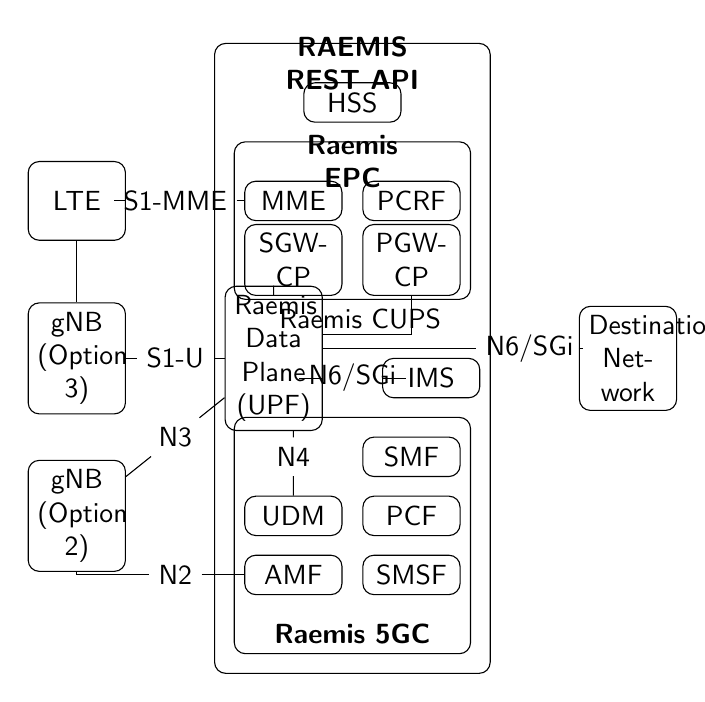
\begin{tikzpicture}[
      node distance=4cm,
      stage/.style={scale=0.75},
      every arrow/.style={thick,>=stealth},
      data/.style={midway, above, font=\small}
    ]

    % Nodes
    \draw[rounded corners] (-1.75, -4) rectangle (1.75, 4);
    \node[align=center, text width=2cm, font=\bfseries] at (0, 3.75) (raemis) {RAEMIS REST API};

    \node[align=center, text width=1cm, draw, rounded corners, minimum height=1cm] (dataplane) at (-1, 0) {Raemis Data Plane (UPF)};

    \node[align=center, text width=1cm, draw, rounded corners,  minimum width=1cm, minimum height=0.5cm] (ims) at (1, -0.25) {IMS};

    \node[align=center, text width=1cm, draw, rounded corners,  minimum width=1cm, minimum height=0.5cm] (hss) at (0, 3.25) {HSS};

    % Raemis EPC
    \node[align=center, text width=1cm, draw, rounded corners, minimum width=3cm, minimum height=2cm, inner ysep=5pt] (epc) at (0, 1.75) {};

    \node[align=center, text width=2cm, font=\bfseries] at (0, 2.5) {Raemis EPC};

    \node[align=center, text width=1cm, draw, rounded corners,  minimum width=1cm, minimum height=0.5cm] (mme) at (-0.75, 2) {MME};

    \node[align=center, text width=1cm, draw, rounded corners,  minimum width=1cm, minimum height=0.5cm] (sgwcp) at (-0.75, 1.25) {SGW-CP};

    \node[align=center, text width=1cm, draw, rounded corners,  minimum width=1cm, minimum height=0.5cm] (pcrf) at (0.75, 2) {PCRF};

    \node[align=center, text width=1cm, draw, rounded corners,  minimum width=1cm, minimum height=0.5cm] (pgwcp) at (0.75, 1.25) {PGW-CP};

    % Raemis 5GC
    \node[align=center, text width=1cm, draw, rounded corners, minimum width=3cm, minimum height=3cm, inner ysep=5pt] (5gc) at (0, -2.25) {};

    \node[align=center, text width=2cm, font=\bfseries] at (0, -3.5) {Raemis 5GC};

    \node[align=center, text width=1cm, draw, rounded corners,  minimum width=1cm, minimum height=0.5cm] (udm) at (-0.75, -2) {UDM};

    \node[align=center, text width=1cm, draw, rounded corners,  minimum width=1cm, minimum height=0.5cm] (amf) at (-0.75, -2.75) {AMF};

    \node[align=center, text width=1cm, draw, rounded corners,  minimum width=1cm, minimum height=0.5cm] (smf) at (0.75, -1.25) {SMF};

    \node[align=center, text width=1cm, draw, rounded corners,  minimum width=1cm, minimum height=0.5cm] (pcf) at (0.75, -2) {PCF};

    \node[align=center, text width=1cm, draw, rounded corners,  minimum width=1cm, minimum height=0.5cm] (smsf) at (0.75, -2.75) {SMSF};

    % Radio Stations

    \node[align=center, text width=1cm, draw, rounded corners, minimum height=1cm] (lte) at (-3.5, 2) {LTE};

    \node[align=center, text width=1cm, draw, rounded corners, minimum height=1cm] (gnb3) at (-3.5, 0) {gNB\\(Option 3)};

    \node[align=center, text width=1cm, draw, rounded corners, minimum height=1cm] (gnb2) at (-3.5, -2) {gNB\\(Option 2)};

    % Destination Network

    \node[align=center, text width=1cm, draw, rounded corners, minimum height=1cm] (dest) at (3.5, 0) {Destination Network};

    % Arrows

    \draw[-] (lte) -- (gnb3);

    \node[align=center] (CUPS) at (0.1, 0.5) {Raemis CUPS};
    \draw[-] (dataplane.north) -- ([xshift=-2.5mm]sgwcp.south);
    \draw[-] ([yshift=0.3cm]dataplane.east) -| (pgwcp);

    \node[align=center] (s1mme) at (-2.25, 2) {S1-MME};
    \draw[-] (lte) -- (s1mme) --(mme);

    \node[align=center] (s1u) at (-2.25, 0) {S1-U};
    \draw[-] (gnb3) -- (s1u) --(dataplane);

    \node[align=center] (n2) at (-2.25, -2.75) {N2};
    \draw[-] (gnb2.south) |- (n2) --(amf);

    \node[align=center] (n3) at (-2.25, -1) {N3};
    \draw[-] (gnb2) -- (n3) --(dataplane);

    \node[align=center] (n4) at (-0.75, -1.25) {N4};
    \draw[-] (udm) -- (n4) --([xshift=0.25cm]dataplane.south);

    \node[align=center] (n6sgi) at (0, -0.25) {N6/SGi};
    \draw[-] (ims) -- (n6sgi) --([yshift=-0.25cm]dataplane.east);

    \node[align=center] (n6sgi) at (2.25, 0.125) {N6/SGi};
    \draw[-] ([yshift=0.125cm]dest.west) -- (n6sgi) --([yshift=0.125cm]dataplane.east);

  \end{tikzpicture}
\end{center}

\begin{itemize}
  \item Raemis UPF implements the standard N3
\end{itemize}

\subsubsection{PDN Functions}

\begin{itemize}
  \item Security and Traffic Segregation
  \item Item Balancing
  \item QoS Allocation
\end{itemize}

\subsubsection{Raemis API}

\begin{itemize}
  \item Exposes a powerful RESTful API that enables application developers to build on top of Raemis or integrate external applications
\end{itemize}

\subsubsection{Raemis GUI}

\begin{itemize}
  \item Uses the Raemis API to access the core software and \textbf{3GPP} components of the network
  \item Hides the complexity of the network
\end{itemize}

\subsection{Grafana}

\begin{itemize}
  \item Open-source Graphite web application (Where Graphite consists of three components: Carbon, Whisper, and Graphite Webapp)
  \item Monitoring tool used for storing and viewing time series data
  \item Multi-platform open source analytics and interactive visualization web application
  \item Produces charts, graphs, alerts, for the web when connected to supported data sources
\end{itemize}

\subsubsection{Data Collection}

\begin{enumerate}
  \item Application writes data to \textbf{JMX beans}
  \item Collectd clients run on all CPS virtual machines such as policy servers and data from \textbf{JMX beans} are collected in case of \textbf{sessionmgr}
  \item Collectd clients push data to collected master node on \textbf{pcrfclient01}
  \item Collectd master node forwards collected data to graphite database on \textbf{pcrfclient01}
  \item The graphite database stores system-related statistics (CPU usage, memory usage, and ethernet interface statistics)
  \item Carbon cache writes this data to Whisper database
  \item Grafana pulls this data from Whisper database configuration and the query is executed in the GUI
\end{enumerate}

\begin{center}
  \vspace{0.4cm}
  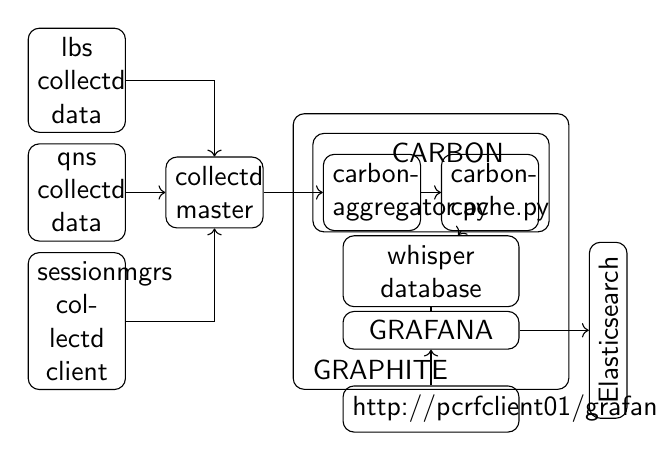
\begin{tikzpicture}[
      node distance=4cm,
      stage/.style={scale=0.75},
      every arrow/.style={thick,>=stealth},
      data/.style={midway, above, font=\small}
    ]
    % Nodes
    \node[align=center, text width=1cm, draw, rounded corners] (master) {collectd master};
    \node[above left=0.3cm and 0.5cm of master, align=center, text width=1cm, draw, rounded corners] (lbsclient) {lbs \\ collectd data};
    \node[left=0.5cm of master, align=center, text width=1cm, draw, rounded corners] (qnsclient) {qns \\ collectd data};
    \node[below left=0.3cm and 0.5cm of master, align=center, text width=1cm, draw, rounded corners] (sessionclient) {sessionmgrs collectd client};

    % Carbon and Graphite
    \draw[rounded corners] (1, 1) rectangle (4.5, -2.5);
    \node[text width=1cm] at (1.75, -2.25) (graphite) {GRAPHITE};
    \draw[rounded corners] (1.25, 0.75) rectangle (4.25, -0.5);
    \node[align=center, text width=1cm] at (2.75, 0.5) (carbon) {CARBON};
    \node[align=center, text width=1cm, draw, rounded corners] (carbona) at (2, 0) {carbon-aggregator.py};
    \node[align=center, text width=1cm, draw, rounded corners] (carbonc) at (3.5, 0){carbon-cache.py};
    \node[align=center, text width=2cm, draw, rounded corners] (whisper) at (2.75, -1){whisper database};
    \node[align=center, text width=2cm, draw, rounded corners] (grafana) at (2.75, -1.75){GRAFANA};
    \node[align=center, text width=2cm, draw, rounded corners] (link) at (2.75, -2.75){http://pcrfclient01/grafana};
    \node[align=center, rotate=90, text width=2cm, draw, rounded corners] (elasticsearch) at (5, -1.75){Elasticsearch};

    % Arrows
    \draw[->] (lbsclient) -| (master);
    \draw[->] (qnsclient) -- (master);
    \draw[->] (sessionclient) -| (master);
    \draw[->] (master) -- (carbona);
    \draw[->] (carbona) -- (carbonc);
    \draw[->] (carbonc) -- (whisper);
    \draw[-] (whisper) -- (grafana);
    \draw[->] (link) -- (grafana);
    \draw[->] (grafana) -- (elasticsearch);
  \end{tikzpicture}
\end{center}

\subsection{OpenNMS Horizon}

\begin{itemize}
  \item Open-source solution that helps visualize and monitor local and remote networks
  \item Offers comprehensive fault, performance, traffic monitoring, and alarm generation
  \item Supports any type of provisioning (auto, directed, topology, etc.)
\end{itemize}

\subsection{Prometheus}

\begin{itemize}
  \item Used for event monitoring and alerting (CPU, RAM, etc.)
  \item Built using an \textbf{HTTP Pull Model} with flexible queries and real-time alerting
  \item Developed at SoundCloud starting 2012
  \item Multi-dimensional data model with time series data identified by metric name and key/value pairs
  \item No reliance on distributed storage
  \item Collected Data can be displayed with \textbf{Grafana}
\end{itemize}

\subsubsection{Architecture}

\begin{center}
  \vspace{0.4cm}
  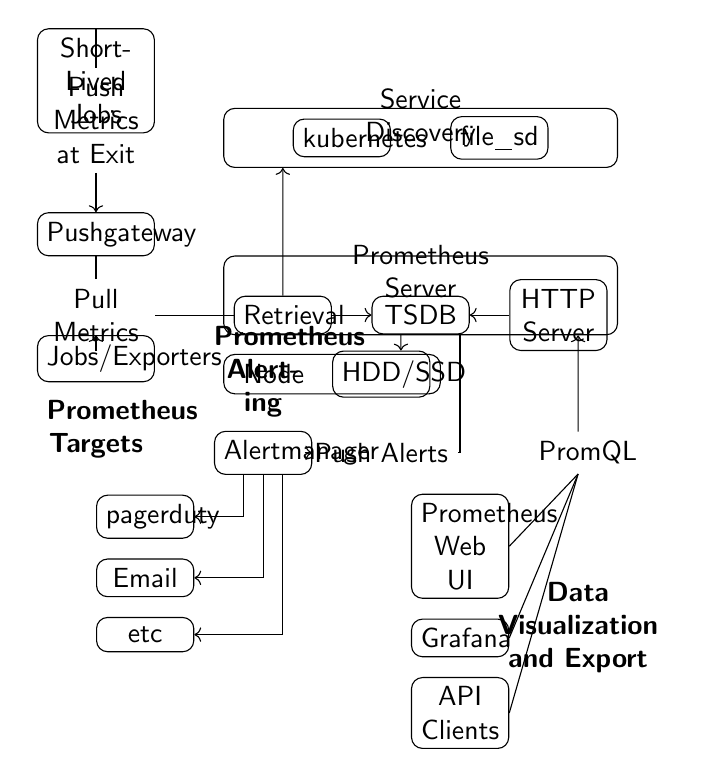
\begin{tikzpicture}[
      node distance=4cm,
      stage/.style={scale=0.75},
      every arrow/.style={thick,>=stealth},
      data/.style={midway, above, font=\small}
    ]

    % Nodes
    \node (rect) at (0, -0.5) [draw, rounded corners, minimum width=5cm, minimum height=1cm](prometheusserver) {};

    \node[align=center, text width=2cm] at (0, -0.2) {Prometheus Server};

    \node[align=center, text width=1cm, draw, rounded corners] at (0, -0.75) (tsdb) {TSDB};

    \node[align=center, text width=1cm, draw, rounded corners] (retrieval) at (-1.75, -0.75) {Retrieval};

    \node[align=center, text width=1cm, draw, rounded corners] (http) at (1.75, -0.75) {HTTP Server};

    \draw[rounded corners]  (-2.5, -1.25) rectangle (0.25, -1.75);
    \node[text width=2cm] at (-1.25, -1.5) {Node};

    \node[align=center, text width=1cm, draw, rounded corners] at (-0.5, -1.5) (hddsdd) {HDD/SSD};

    \node (rect) at (0, 1.5) [draw, rounded corners, minimum width=5cm, minimum height=0.75cm] (servicediscovery) {};

    \node[align=center, text width=2cm] at (0, 1.75) {Service Discovery};

    \node[align=center, text width=1cm, draw, rounded corners] at (-1, 1.5) (kubernetes) {kubernetes};
    \node[align=center, text width=1cm, draw, rounded corners] at (1, 1.5) (filesd) {file_sd};

    \node[above left = 0.5cm and 1cm of retrieval, align=center, text width=1.25cm, draw, rounded corners] (pushgateway) {Pushgateway};

    \node[below = 1cm of pushgateway, align=center, text width=1.25cm, draw, rounded corners] (jobs) {Jobs/Exporters};

    \node[below = 0.1cm of jobs, font=\bfseries, align=center, text width=1.25cm] {Prometheus Targets};

    \node[above = 0.5cm of pushgateway, align=center, text width=1.5cm] (pushmetrics) {Push Metrics at Exit};

    \node[above = 1cm of pushgateway, align=center, text width=1.25cm, draw, rounded corners] (shortjobs) {Short-Lived Jobs};

    \node[align=center, text width=1cm, draw, rounded corners] at (-2, -2.5) (alertmanager) {Alertmanager};

    \node[below left = 0.25cm and 0.25cm of alertmanager, align=center, text width=1cm, draw, rounded corners](pagerduty) {pagerduty};

    \node[below = 0.25cm of pagerduty, align=center, text width=1cm, draw, rounded corners](email) {Email};

    \node[below = 0.25cm of email, align=center, text width=1cm, draw, rounded corners](etc) {etc};

    \node[align=center, text width=1cm] at (2, -2.5) (promql) {PromQL};

    \node[below left = 0.25cm and 0.25cm of promql, align=center, text width=1cm, draw, rounded corners](webui) {Prometheus Web UI};

    \node[below = 0.25cm of webui, align=center, text width=1cm, draw, rounded corners](grafana) {Grafana};

    \node[below = 0.25cm of grafana, align=center, text width=1cm, draw, rounded corners](api) {API Clients};

    \node[above = 0.05cm of alertmanager, font=\bfseries, align=center, text width=1.25cm] {Prometheus Alerting};

    \node[below = 1.25cm of promql, font=\bfseries, align=center, text width=2.25cm] {Data Visualization\\and Export};

    % Arrows
    \draw[->] (retrieval) -- (tsdb);
    \draw[->] (http) -- (tsdb);
    \draw[->] ([xshift=-0.25cm]tsdb.south) -- ([xshift=0.25cm]hddsdd.north);
    \draw[->] (retrieval) -- ([xshift=-1.75cm]servicediscovery.south);

    \node[left = 1cm of retrieval, align=center, text width=1.25cm] (pullmetrics) {Pull Metrics};
    \draw[-] (retrieval) -- (pullmetrics) -- (pushgateway);
    \draw[->] (pullmetrics) -- (jobs);

    \draw[-] (shortjobs) -- (pushmetrics);
    \draw[->] (pushmetrics) -- (pushgateway);

    \node[align=center] at (-0.5, -2.5) (pushalerts) {Push Alerts};
    \draw[->] ([xshift=0.5cm] prometheusserver.south) |- (pushalerts) -- (alertmanager);

    \draw[->] ([xshift=-0.25cm]alertmanager.south) |- (pagerduty.east);
    \draw[->] (alertmanager.south) |- (email.east);
    \draw[->] ([xshift=0.25cm]alertmanager.south) |- (etc.east);

    \draw[->] (promql.north) -- ([xshift=2cm] prometheusserver.south);

    \draw[-] (webui.east) -- (promql.south);
    \draw[-] (grafana.east) -- (promql.south);
    \draw[-] (api.east) -- (promql.south);

  \end{tikzpicture}

\end{center}

\subsection{Windows 11}

\begin{itemize}
  \item Current latest major Microsoft's Windows NT OS
  \item Major changes to the Windows shell, which was influenced by Windows 10X, a canceled deluxe edition to Windows 10
  \item Redesigned Start menu, replacement of "live tiles" with a separate "Widgets" panel in the taskbar, etc.
\end{itemize}

\subsection{Windows Server 2025}

\begin{itemize}
  \item Server-oriented releases of Windows NT OS
  \item Uses \textbf{SMB} instead of \textbf{QUIC}
  \item Compared to Windows, this is used for network servers, whereas base Windows 11 is used for desktop computers and personal use
  \item New features such as Bluetooth connection, DTrace, and additional emails and accounts
\end{itemize}

\section{Configurations}

\begin{center}
  \begin{tabular}{| m{2cm} | m{6cm} |}
    \hline
    \textbf{2oo2} & Requires both signals to agree to trigger a shutdown.    \\
    \hline
    \textbf{2oo3} & Requires two out of three signals to trigger a shutdown. \\
    \hline
    \textbf{3oo3} & Requires all three signals to trigger a shutdown.        \\
    \hline
  \end{tabular}
\end{center}
\end{multicols*}

\end{document}